\section{Detailed Results}
\label{sec:benchs-pres}

In this section we show the results of the competition from the benchmark's perspective.
For a given benchmark we would like to know:
\begin{inlist}
	\item how many solvers solved it
	\item what are the minimum and maximum times required to solve
	\item what are the minimum and maximum sizes of solutions generated
	\item which solver solved the benchmark the fastest, and
	\item which solver produced the smallest expression.
\end{inlist}

We represents the results per benchmark in groups organized per tracks and categories.
For instance, the top plot in \Cref{fig:prog-rep-icfp} presents the details for program repair benchmarks from the general track.
The black bars above the $y$-axis show the range of time taken to solve across the various solvers, in our pseudo logarithmic scale.
Inspect for instance benchmark \texttt{t2.sl}.
The black bar indicates that the fastest solver takes less than $1$ second, and the slowest one takes between $100$ to $300$ seconds.
The black number above the black bar indicates the exact number of seconds (floor-rounded to the nearest second)
it took the slowest solver to solve a benchmark (and $\infty$ if at least one solver exceeded the time bound).
Thus, we can see that for \texttt{t2.sl}, the slowest solver took $138$ seconds.
The white number at the lower part of the bar indicates the time taken by the fastest solver.
Thus, we can see that for \texttt{t2.sl}, the fastest solver required less than $1$ second.
The colored squares/rectangles below the black bar indicate which solvers were among the fastest to solve that benchmark
(according to the solvers' legend at the top).
For instance, we can see that \cvcnew\ and \eusolvernew\ were the fastest to solve \texttt{t2.sl},
solving it in less than a second, and that among the solvers that solved \texttt{t4.sl} only \eusolvernew\ solved it in less than a second.

Similarly, the gray bars below the $y$-axis indicate the range of expression sizes in pseudo-logarithmic scales,
where the size of an expression is determined by the number of nodes in its parse tree.
The black number at the bottom of the gray bar indicates the exact size of the largest solution (or $\infty$ if it exceeded $1000$),
and the white number at the top of the gray bar indicates the exact size of the smallest solution.
When the smallest and largest size of expressions are in the same pseudo-logarithmic bucket, as is the case in \texttt{t2.sl}),
we indicate the expression size only in black.
The colored squares/rectangles above the gray bar indicate which solvers were amongst the ones that produced the smallest expression
(according to the solvers' legend at the top).
For instance, for \texttt{t20.sl} the smallest expression produced had size $3$,
which is produced only by \eusolvernew.

Finally, the top $x$-axis of each figure indicates the number of solvers that solved a particular benchmark (on the bottom $x$-axis).
For instance, in \Cref{fig:prog-rep-icfp}, only one solver solved \texttt{t6.sl}, two solvers solved \texttt{t14.sl},
three solvers solved \texttt{t2.sl}, and no solver solved \texttt{t13.sl}.
Note that for the benchmarks that no solver is able to solve, the black bars indicate the range of time taken by solvers to terminate.
When no solver produces a correct result, there are no colored squares/rectangles below the black bars, as is the case for \texttt{t13.sl}.


\begin{figure*}
	\noindent\makebox[\textwidth]{
		\scalebox{0.625}{
			\begin{tabular}{c}
				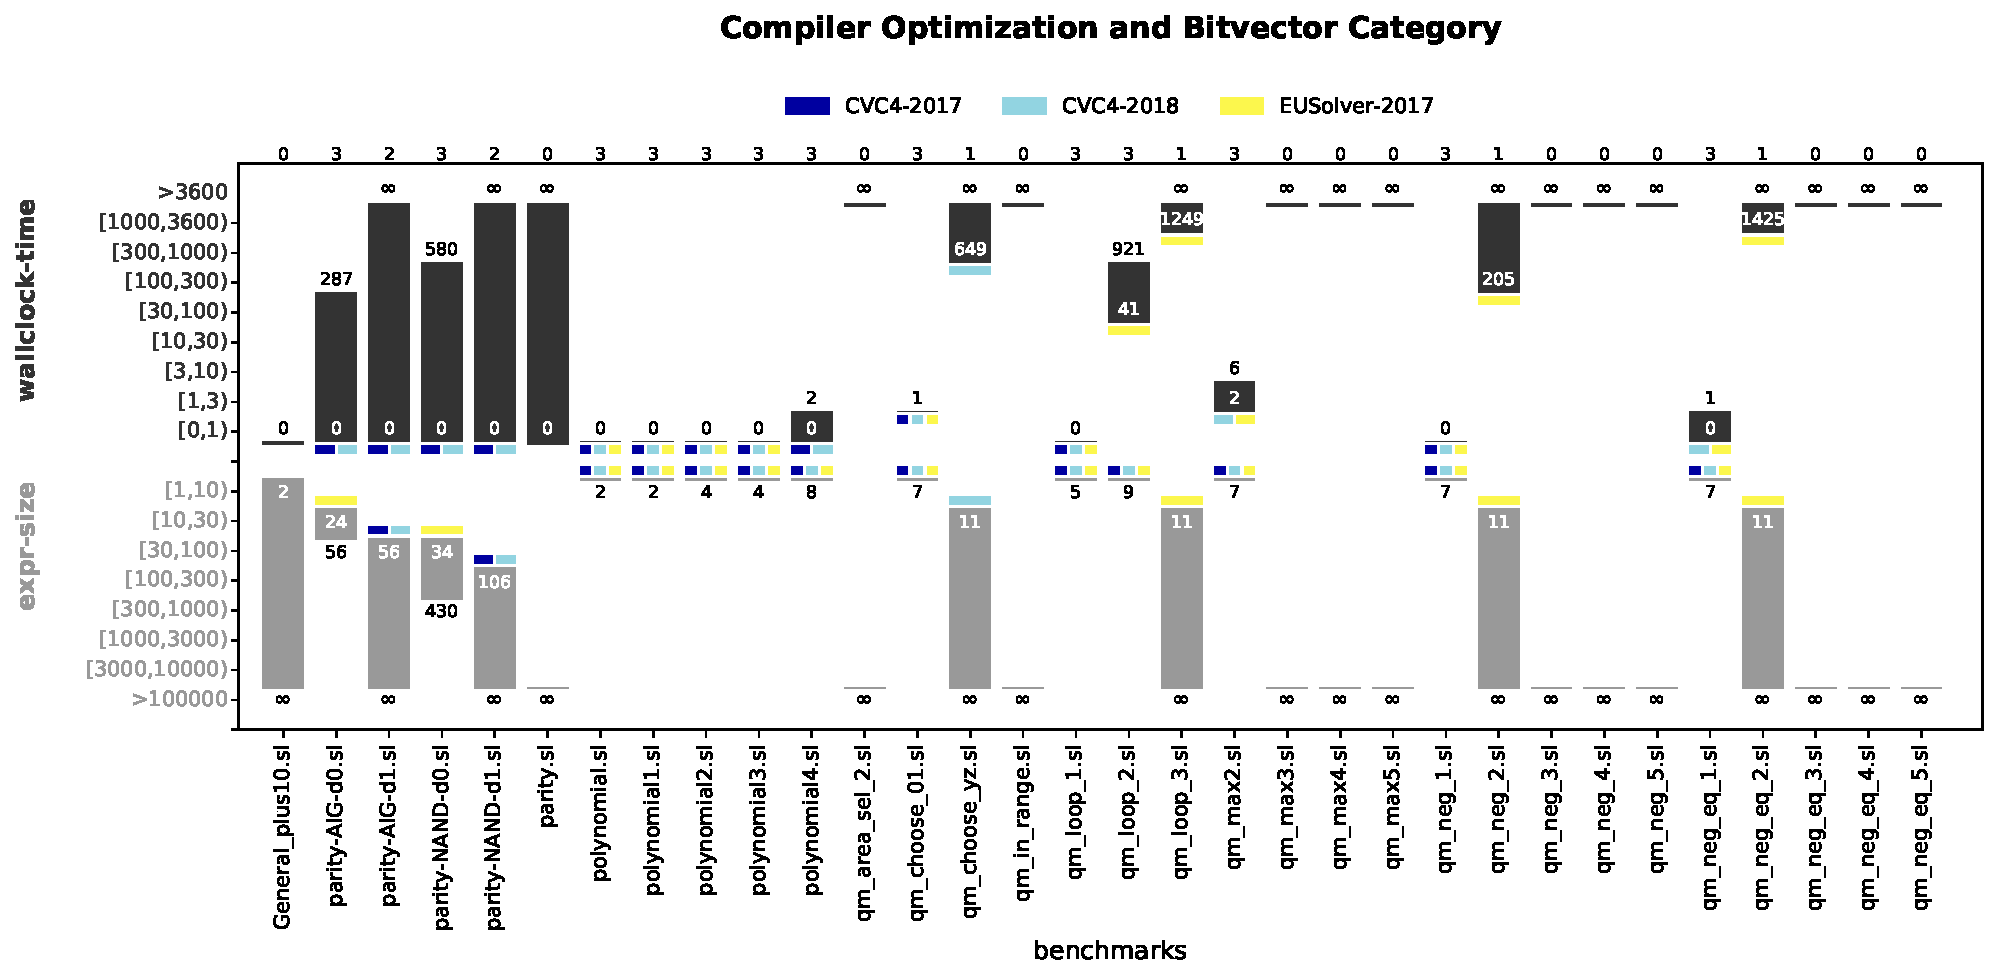
\includegraphics[width=10in]{figures/General1.pdf} \\[3cm]
				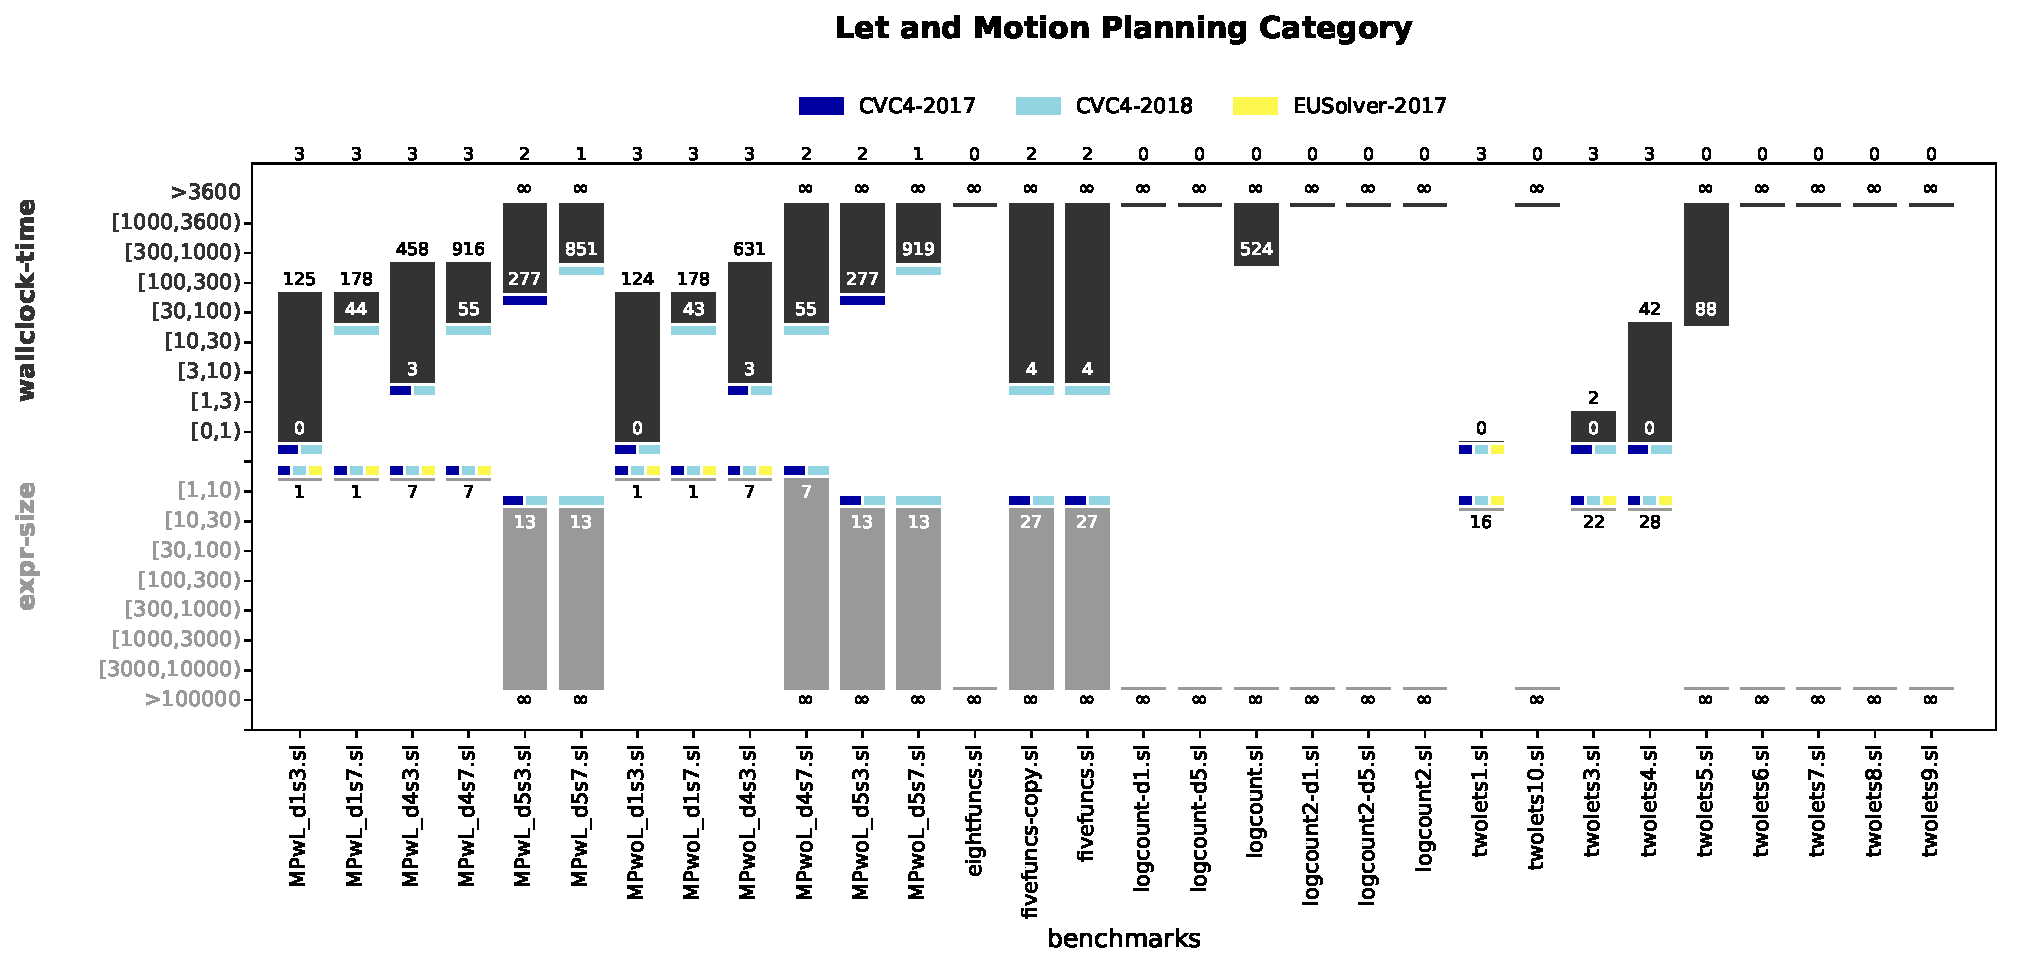
\includegraphics[width=10in]{figures/General2.pdf}
			\end{tabular}
	}}
	\caption{Evaluation of compiler optimizations, bitvectors, let and motion planning,
			 and program repair categories of the General track.}
	\label{fig:let-mot-plan}
\end{figure*}

\begin{figure*}
	\noindent\makebox[\textwidth]{
		\scalebox{0.625}{
			\begin{tabular}{c}
				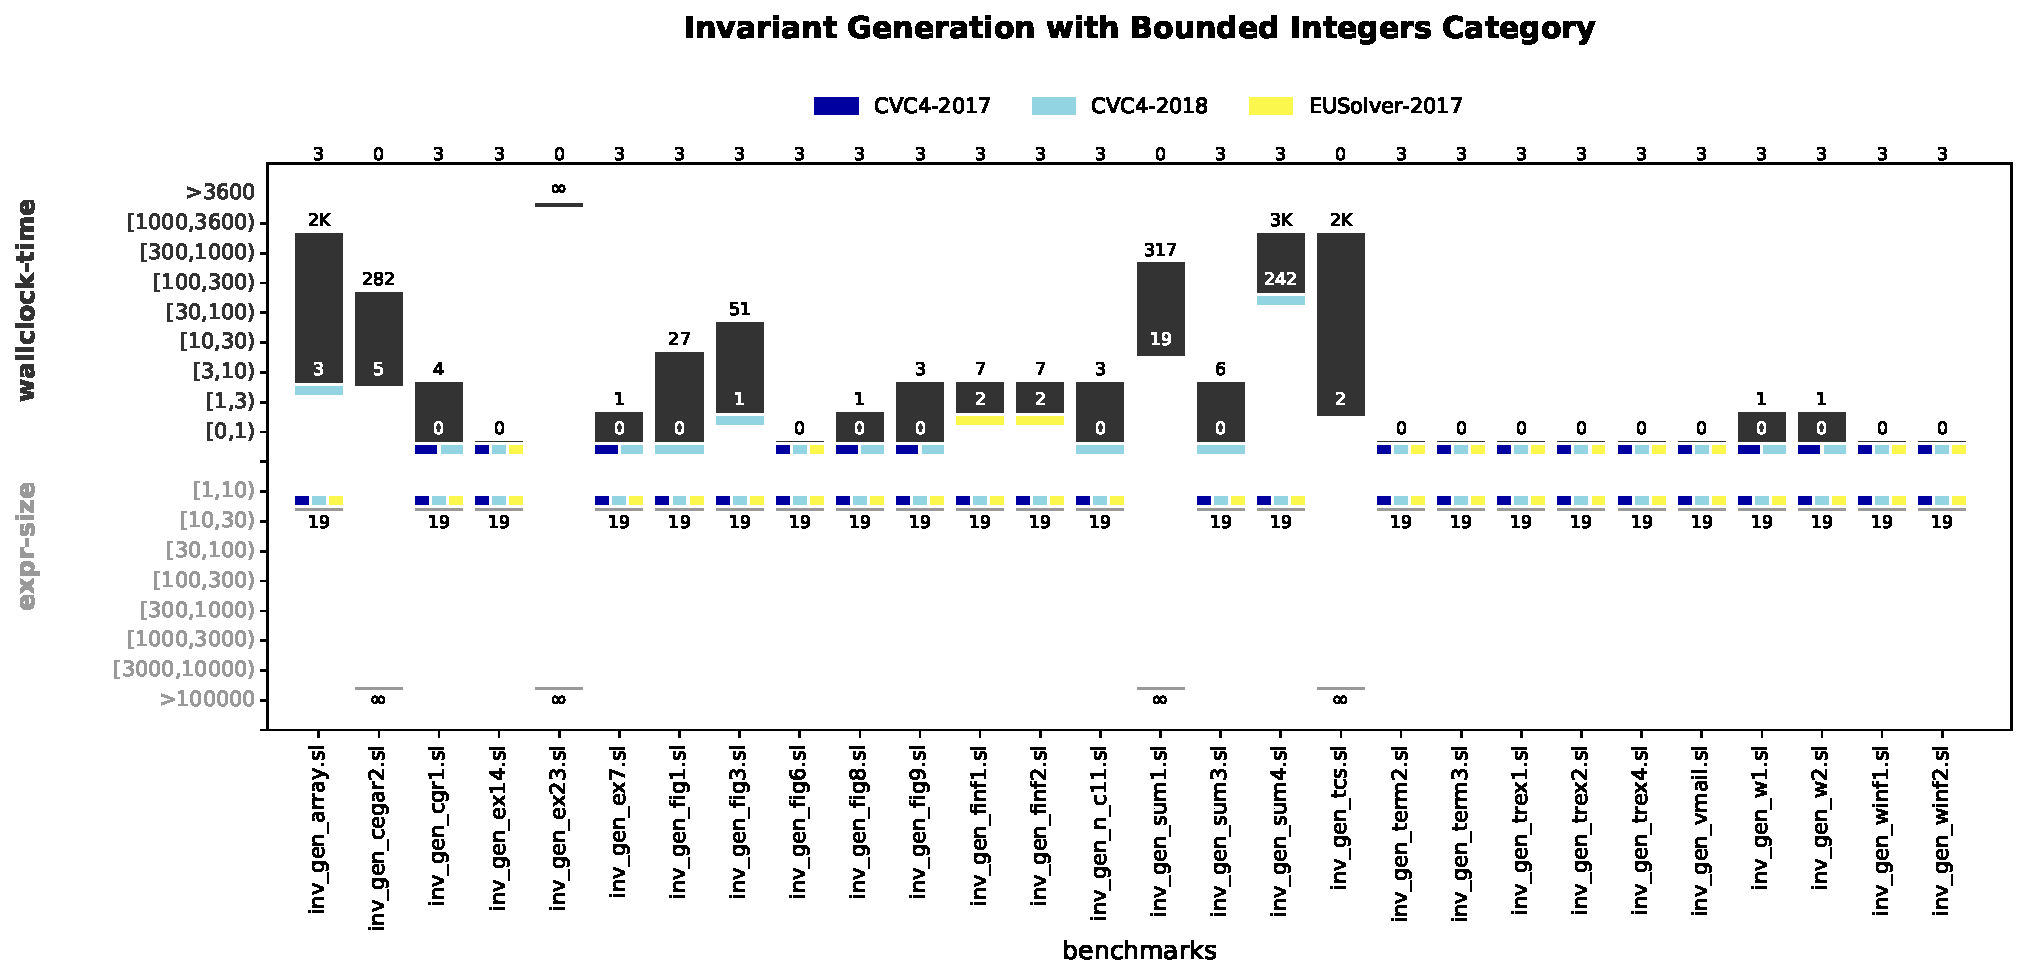
\includegraphics[width=10in]{figures/General3.pdf} \\[3cm]
				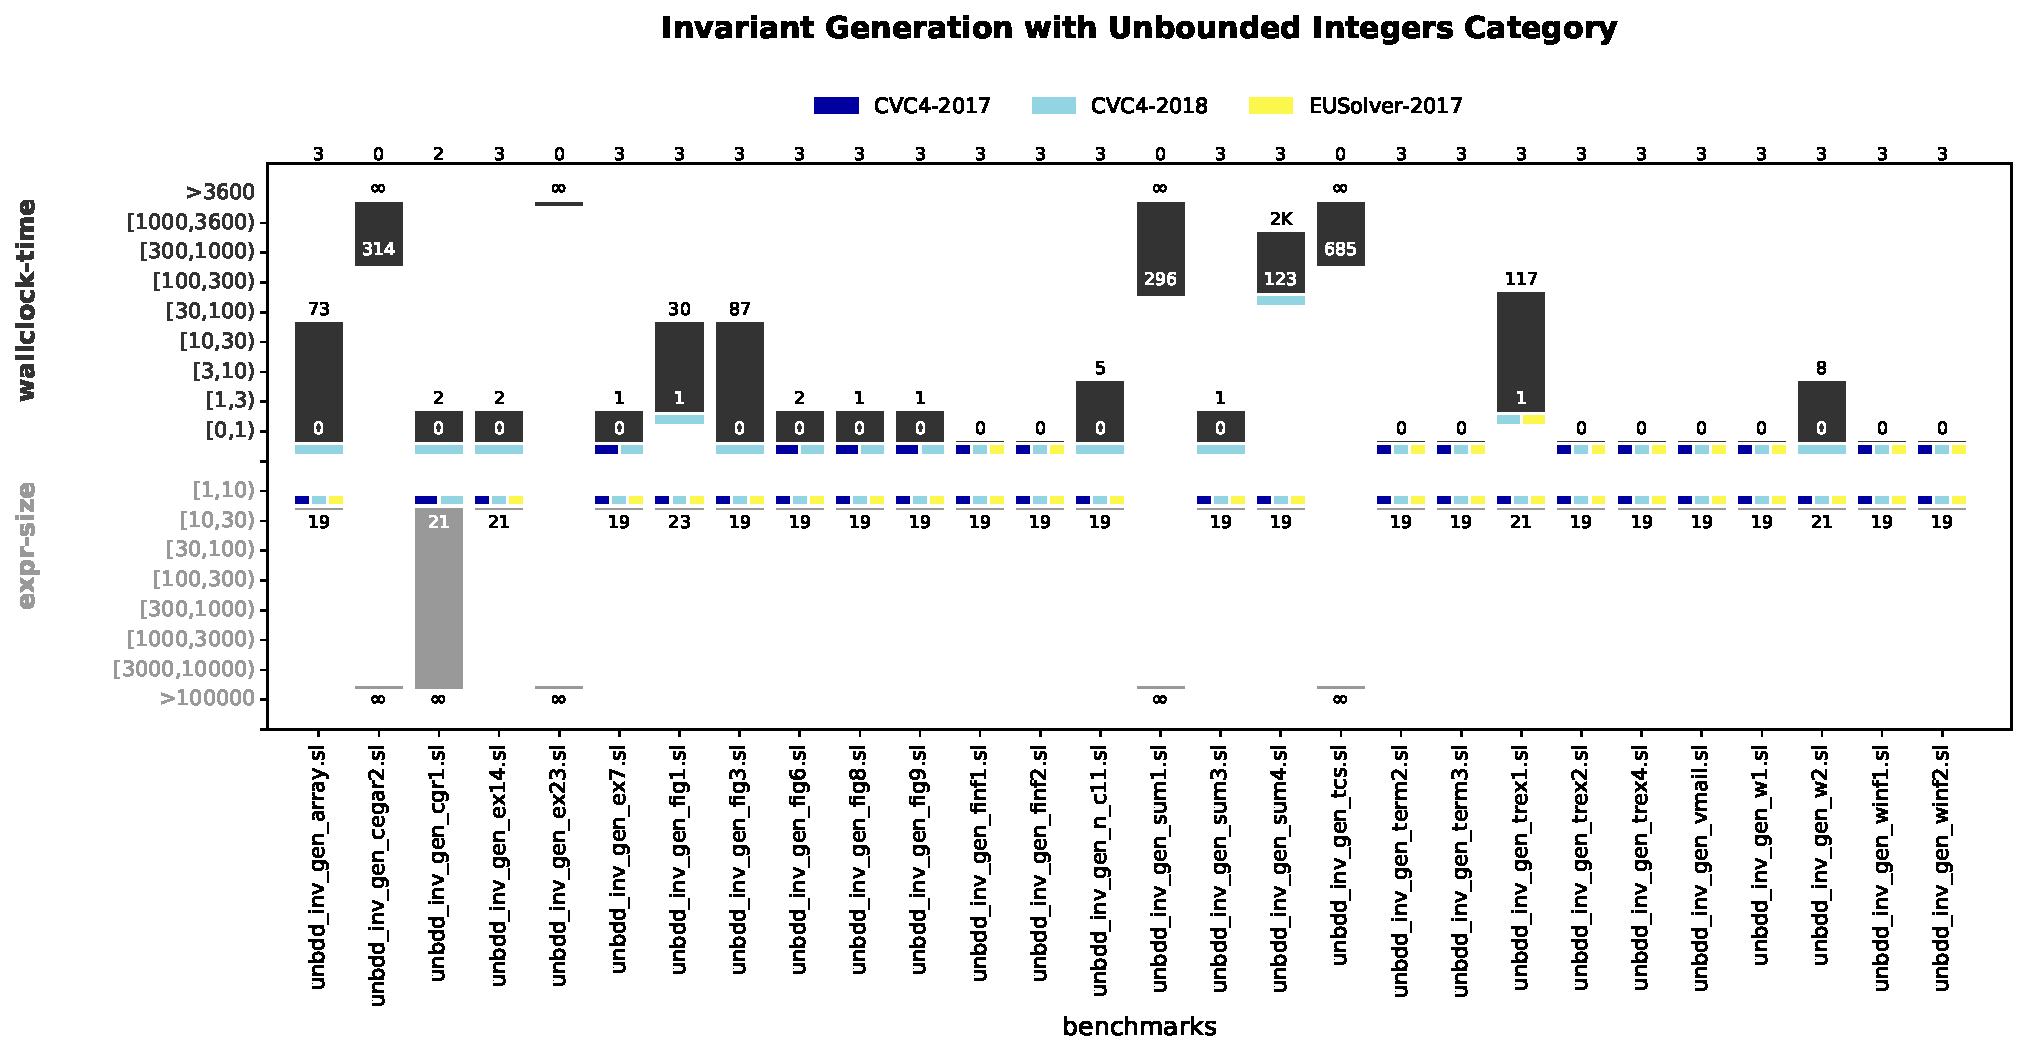
\includegraphics[width=10in]{figures/General4.pdf} 
			\end{tabular}
	}}
	\caption{Evaluation of invariant generation categories of the General track.}
	\label{fig:inv-results}
\end{figure*}

\begin{figure*}
	\noindent\makebox[\textwidth]{
		\scalebox{0.625}{
			\begin{tabular}{c}
				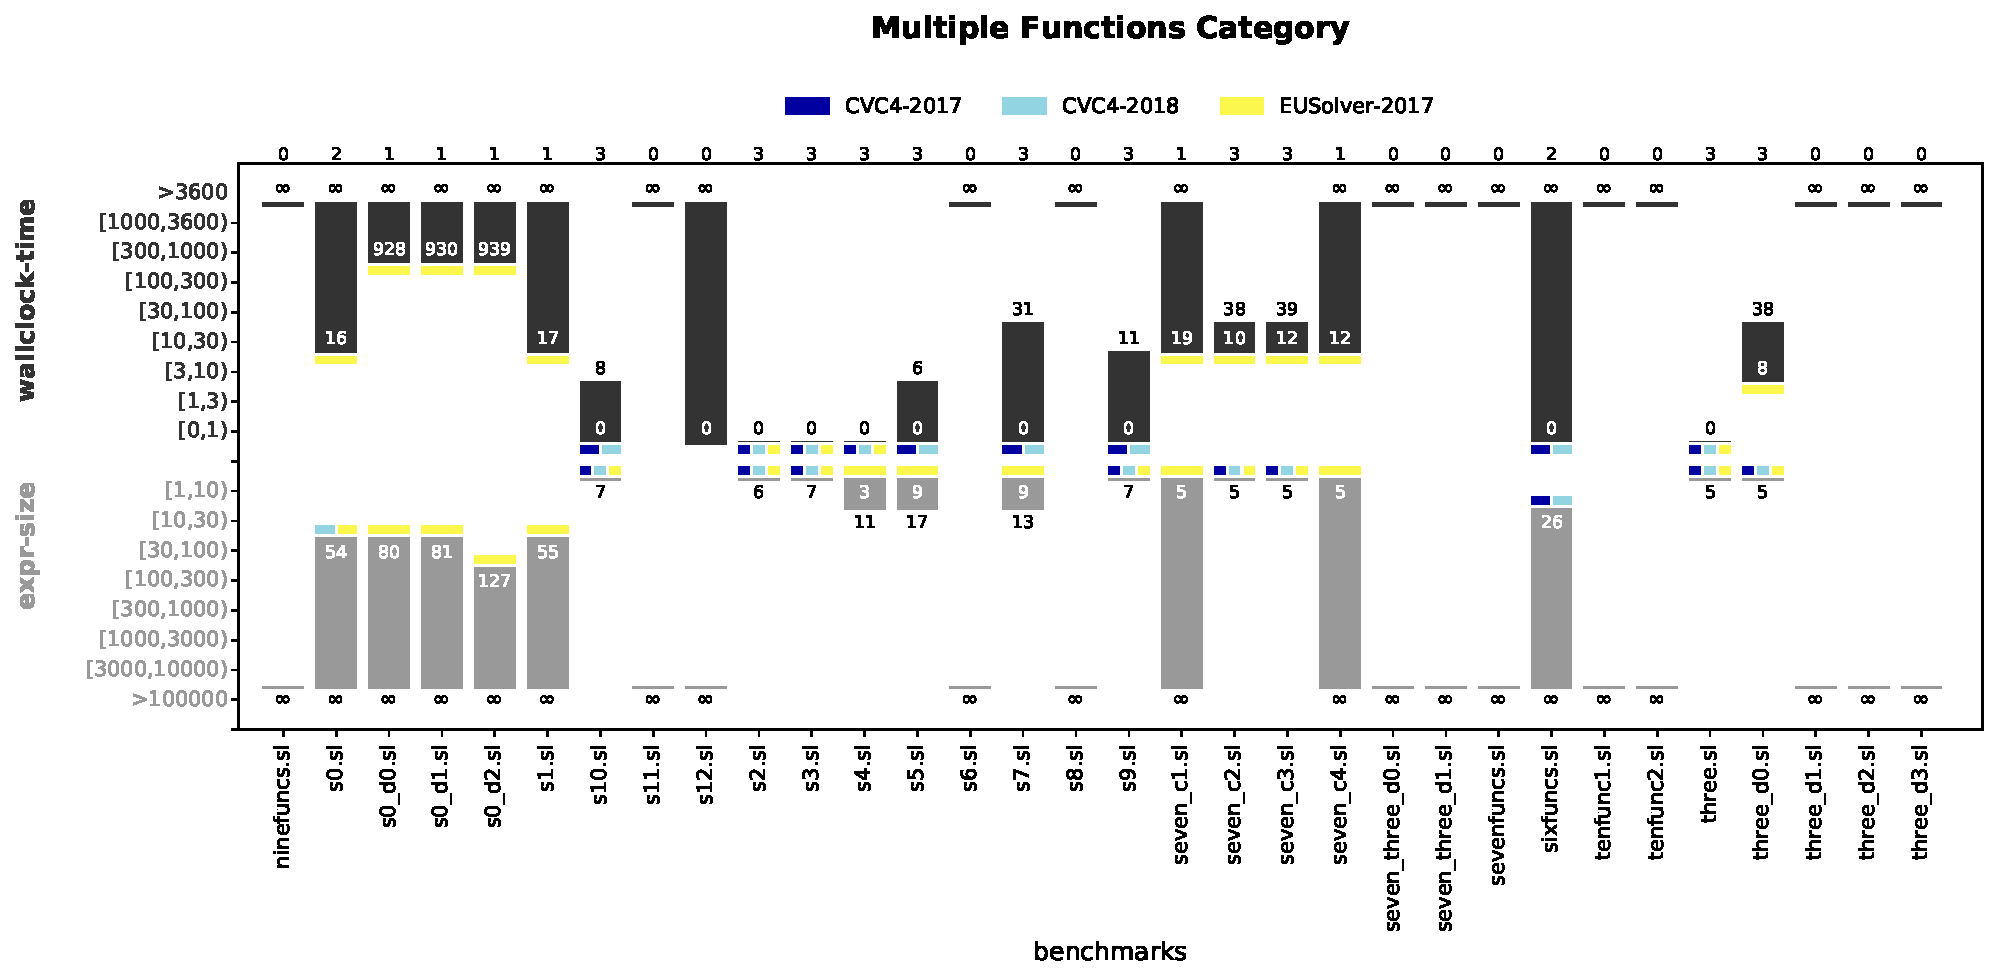
\includegraphics[width=10in]{figures/General5.pdf} \\[3cm]
				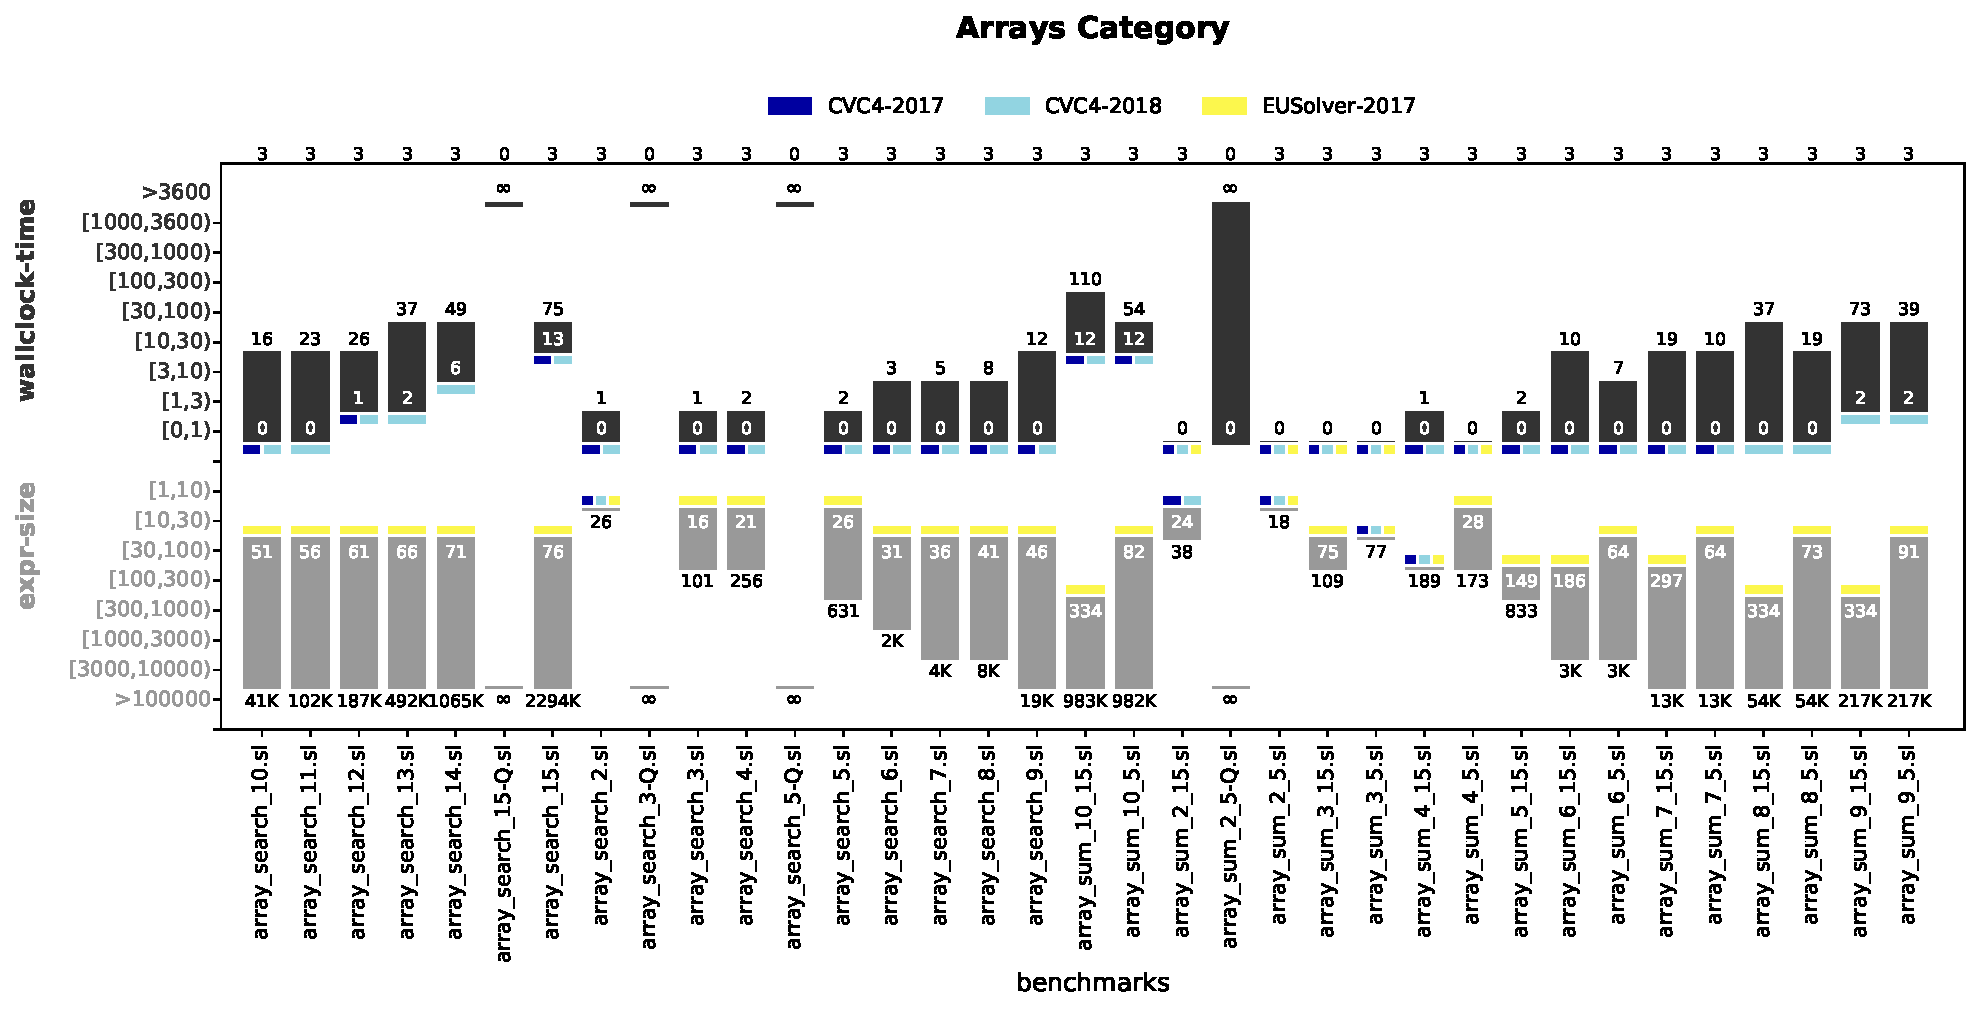
\includegraphics[width=10in]{figures/General6.pdf} 
			\end{tabular}
	}}
	\caption{Evaluation of multiple functions and arrays categories of the General track.}
	\label{fig:mult-func-arr}
\end{figure*}

\begin{figure*}
	\noindent\makebox[\textwidth]{
		\scalebox{0.6}{
			\begin{tabular}{c}
				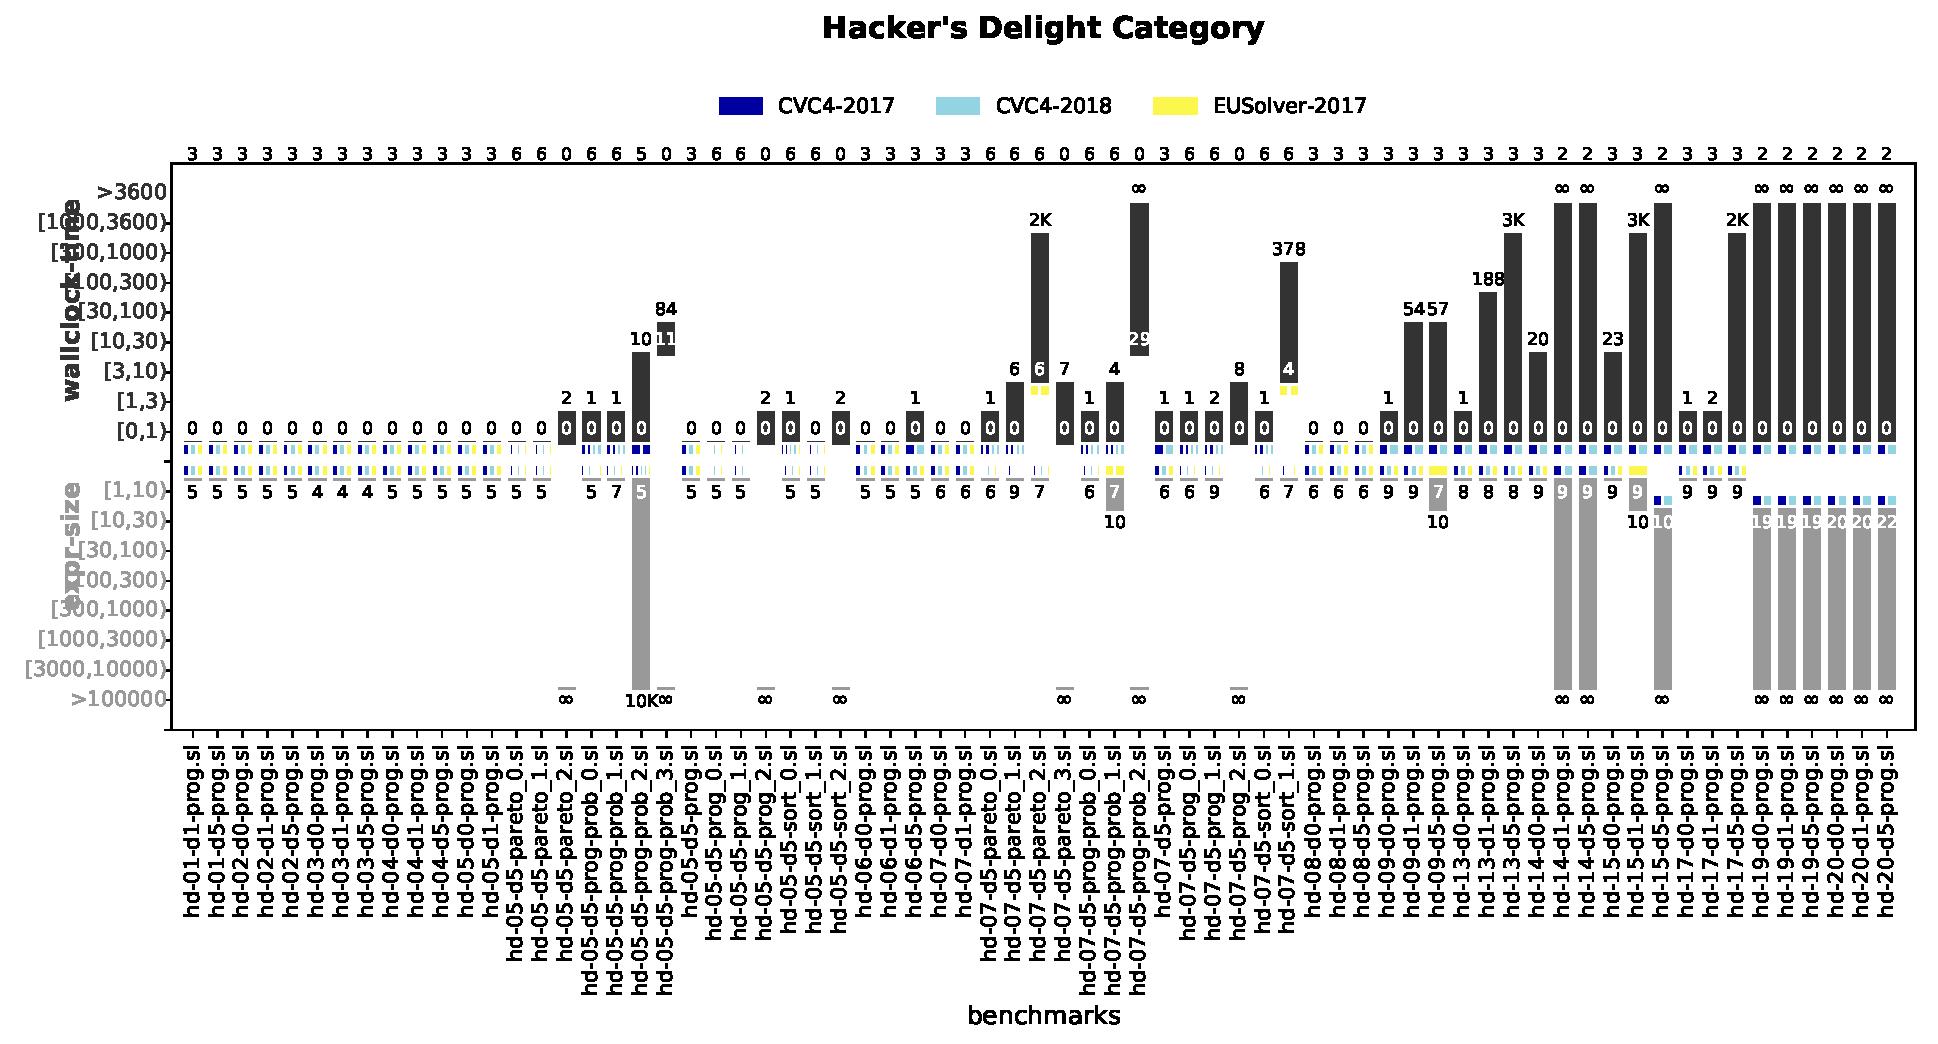
\includegraphics[width=10in]{figures/General7.pdf} \\[3cm]
				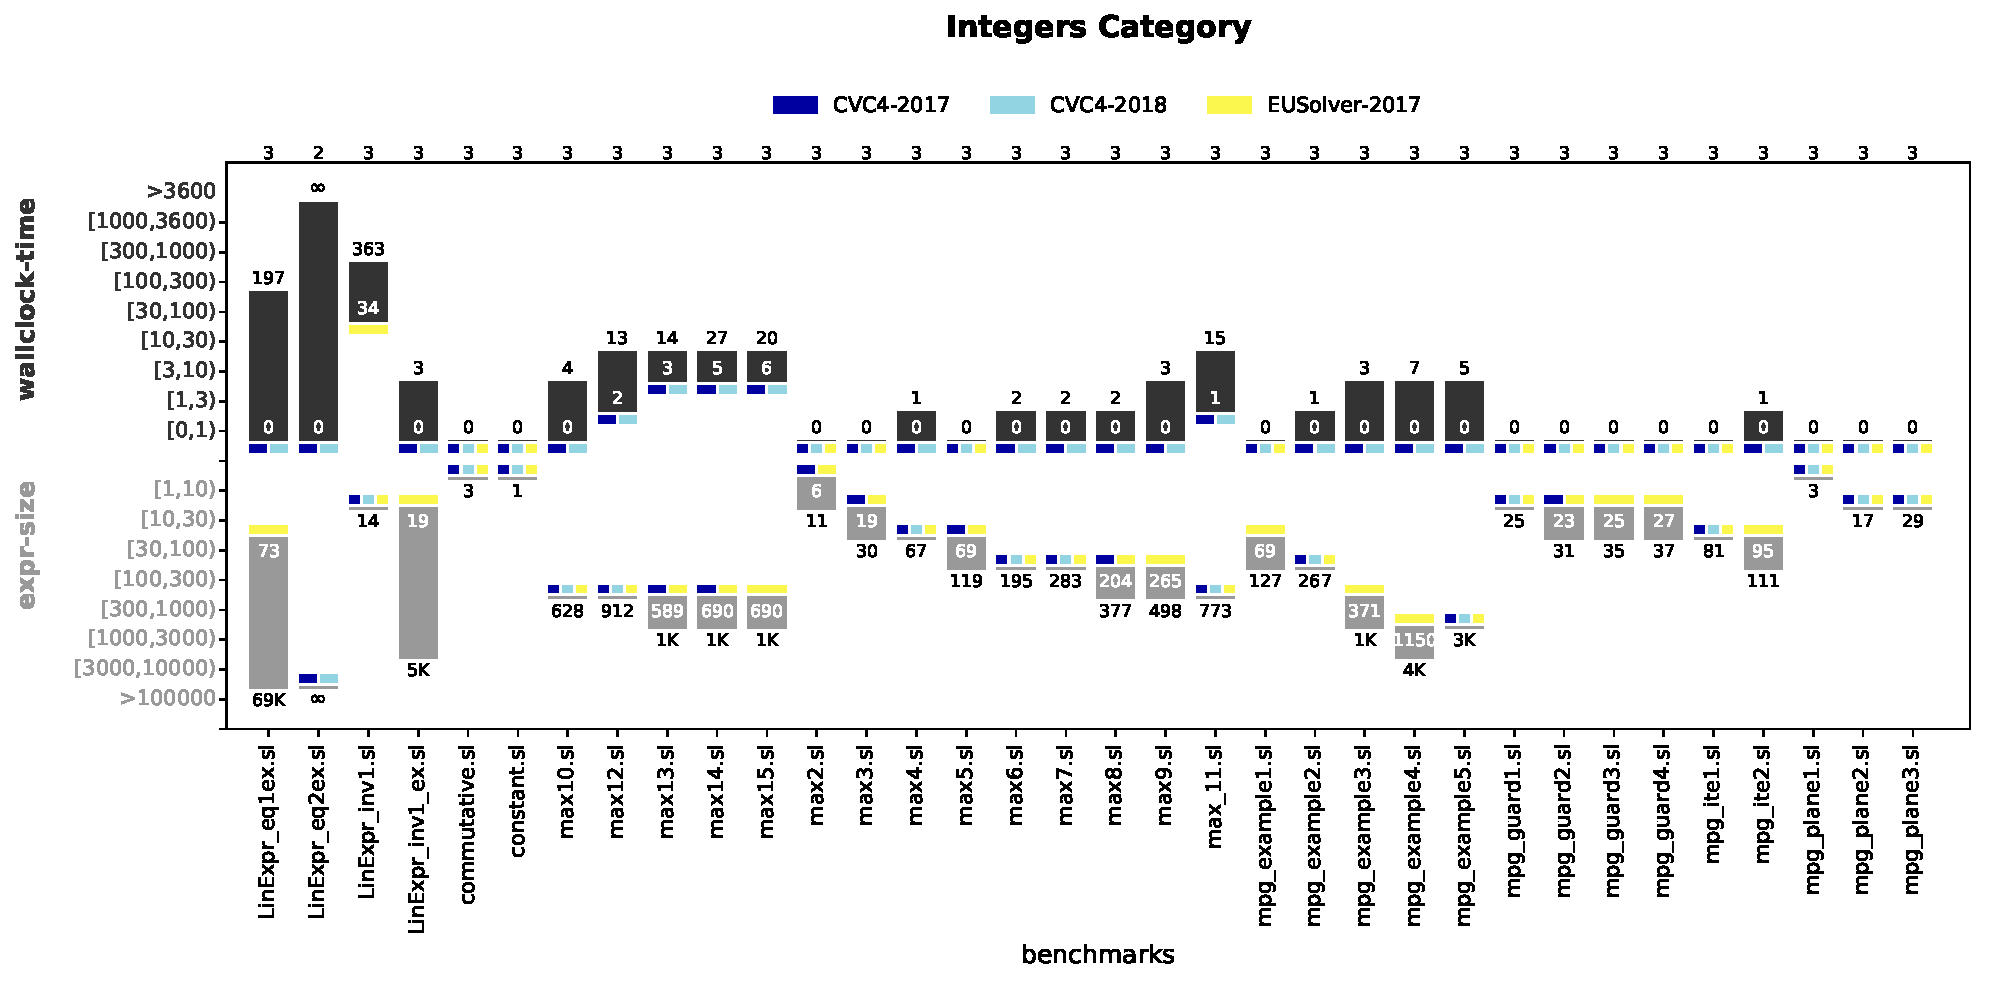
\includegraphics[width=10in]{figures/General8.pdf} 
			\end{tabular}
	}}
	\caption{Evaluation of hacker's delight and integers categories of the General track.}
	\label{fig:hd-int}
\end{figure*}

\begin{figure*}
	\noindent\makebox[\textwidth]{
		\scalebox{0.625}{
			\begin{tabular}{c}
				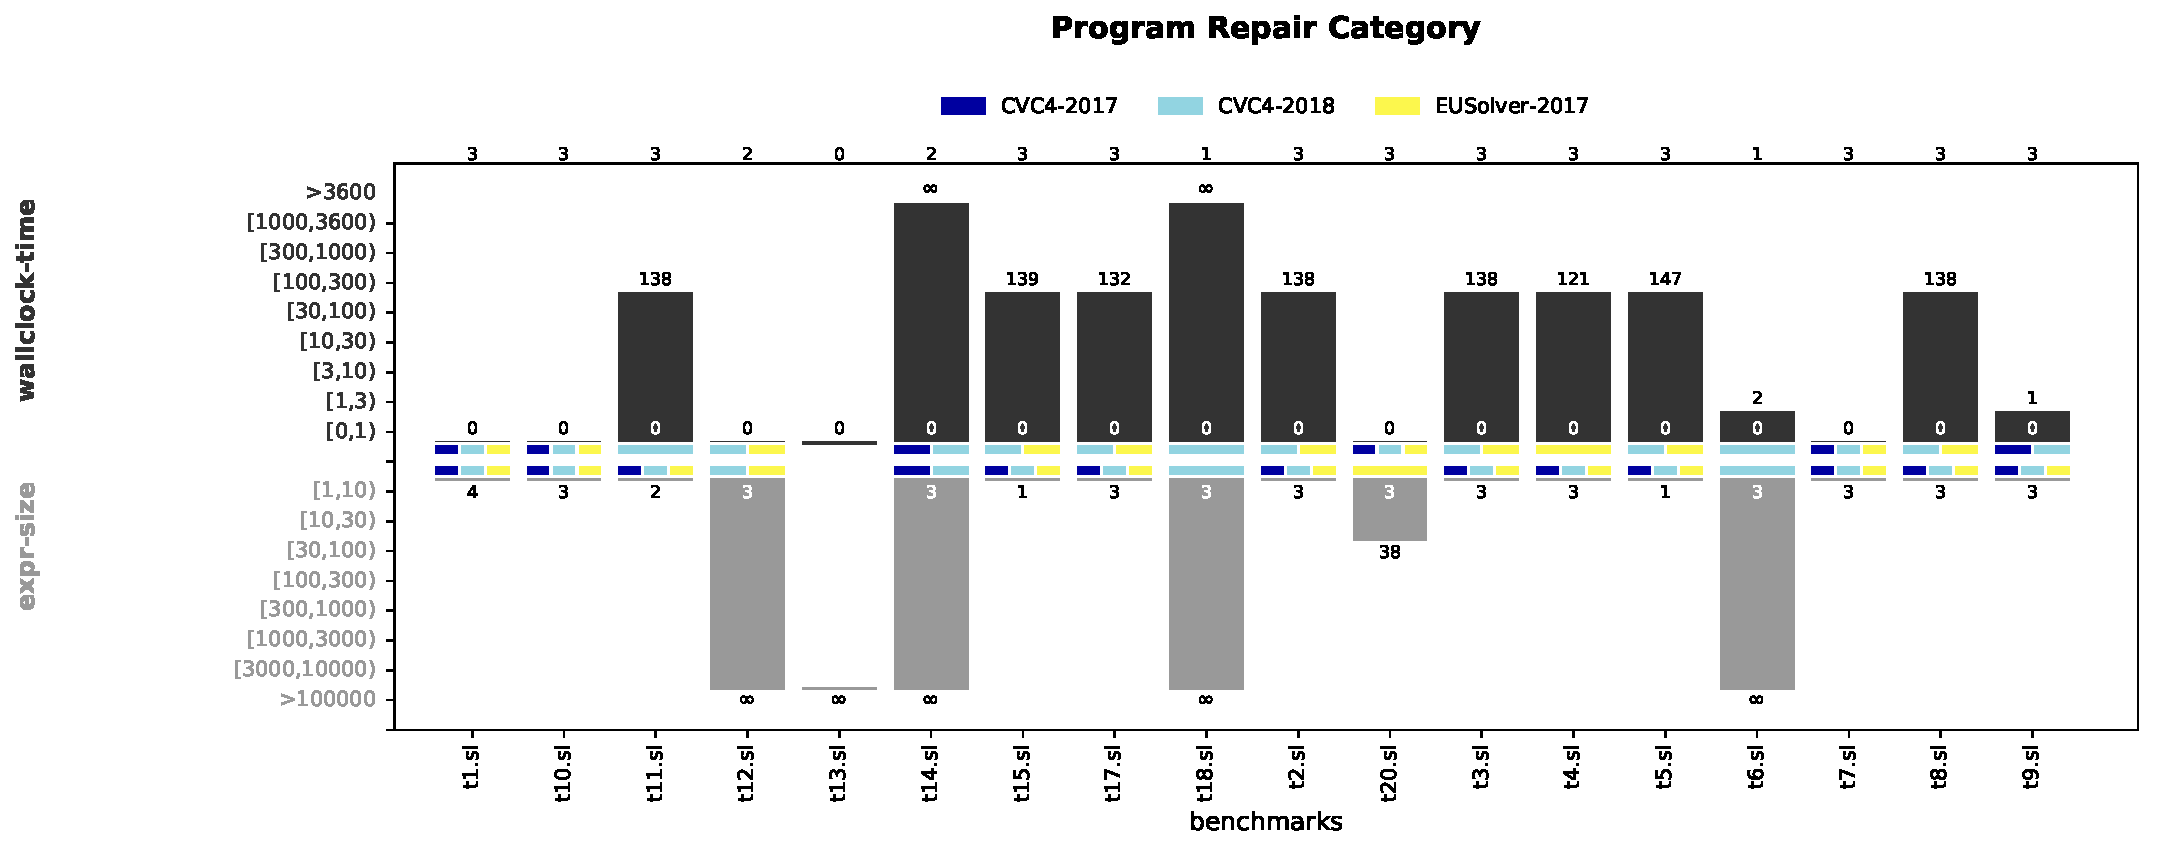
\includegraphics[width=10in]{figures/General9.pdf} \\[3cm]
				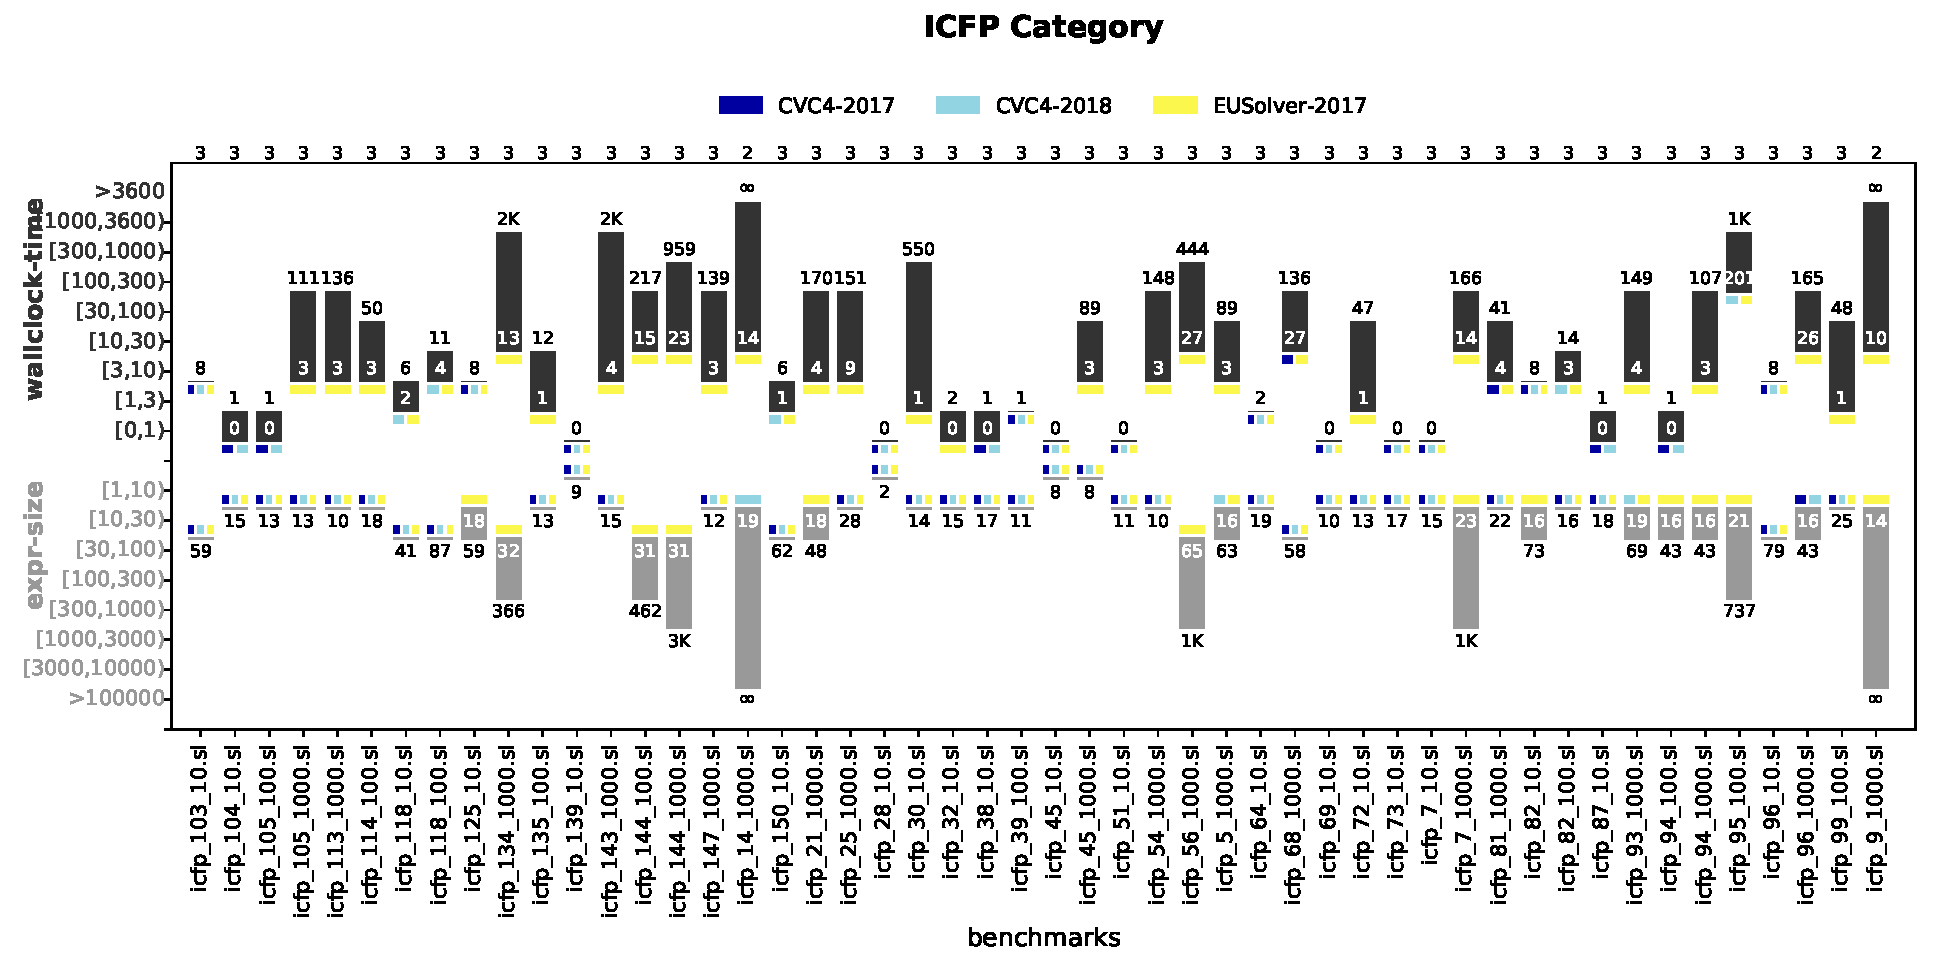
\includegraphics[width=10in]{figures/General10.pdf}
			\end{tabular}
	}}
	\caption{Evaluation of program repair and ICFP categories of the General track.}
	\label{fig:prog-rep-icfp}
\end{figure*}

\begin{figure*}
	\noindent\makebox[\textwidth]{
		\scalebox{0.625}{
			\begin{tabular}{c}
				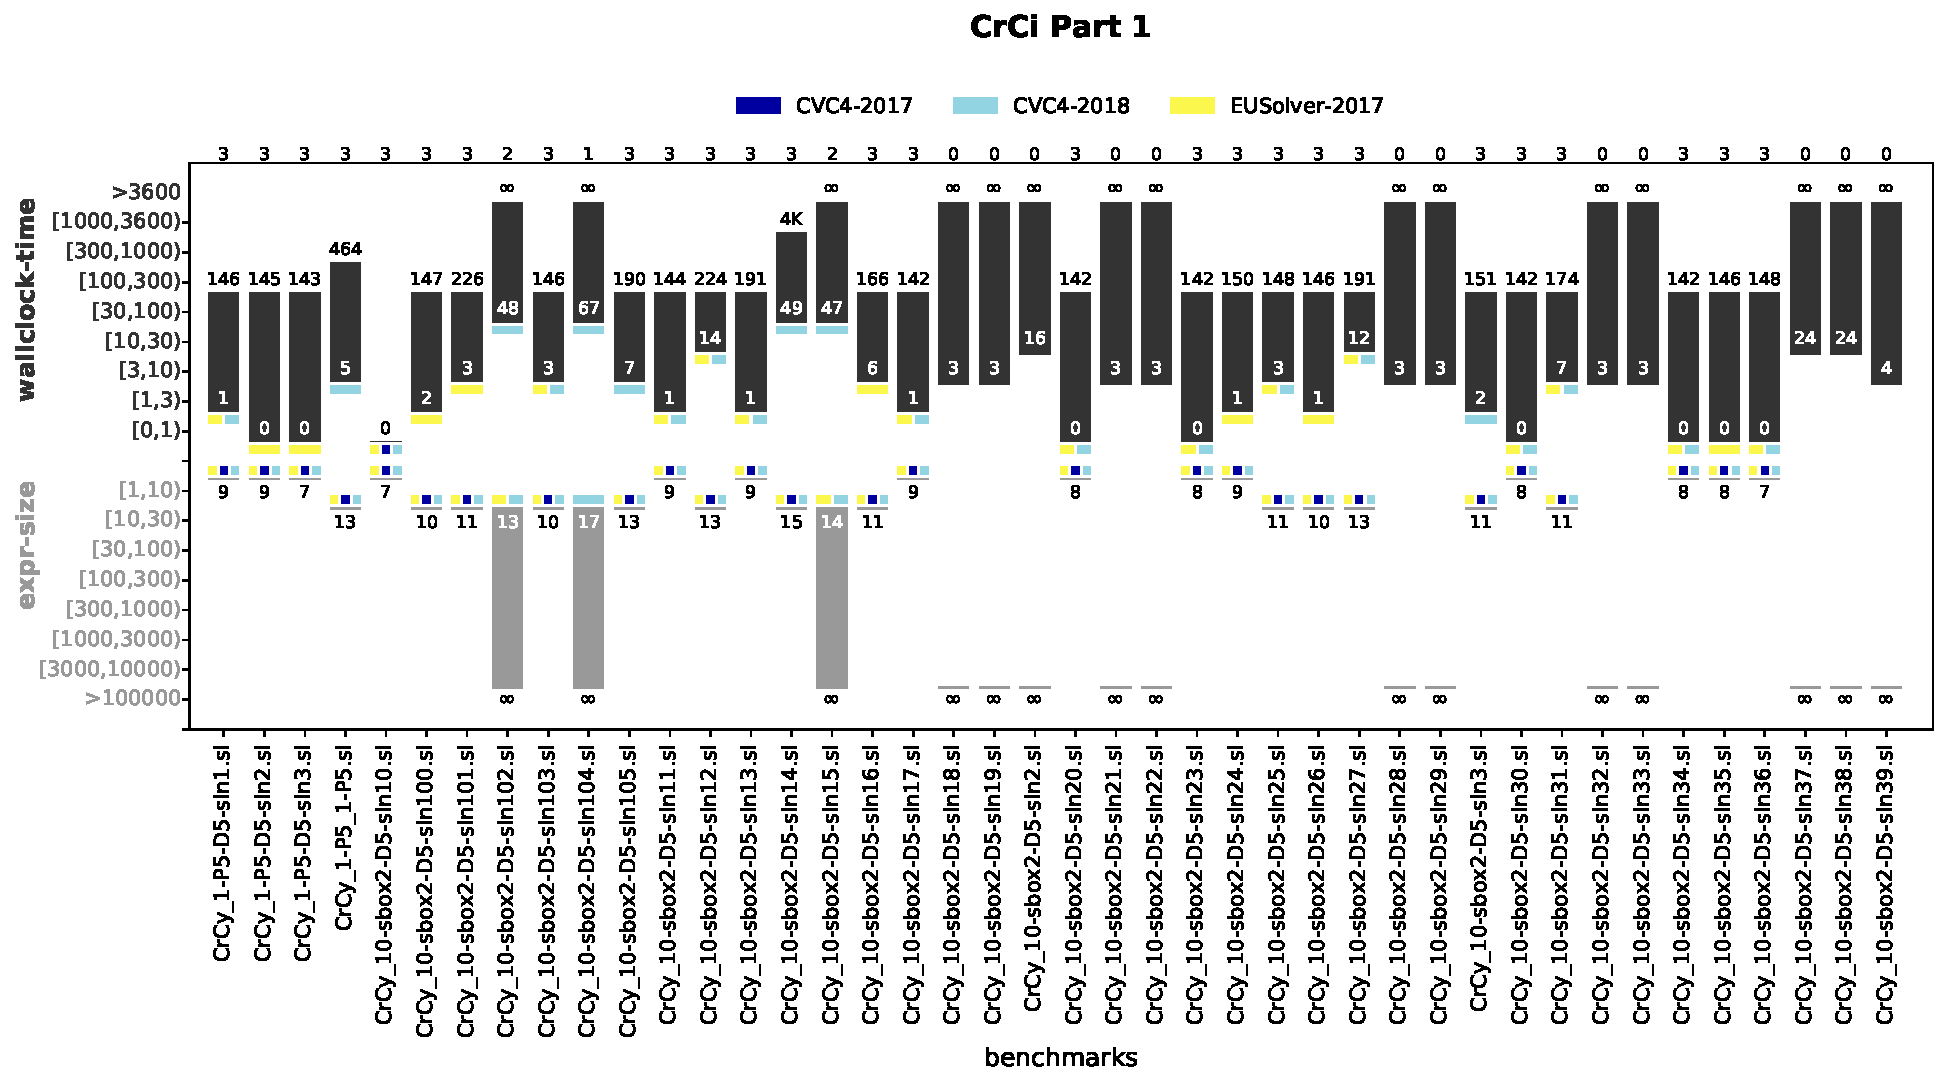
\includegraphics[width=10in]{figures/CrCi1.pdf} \\[3cm]
				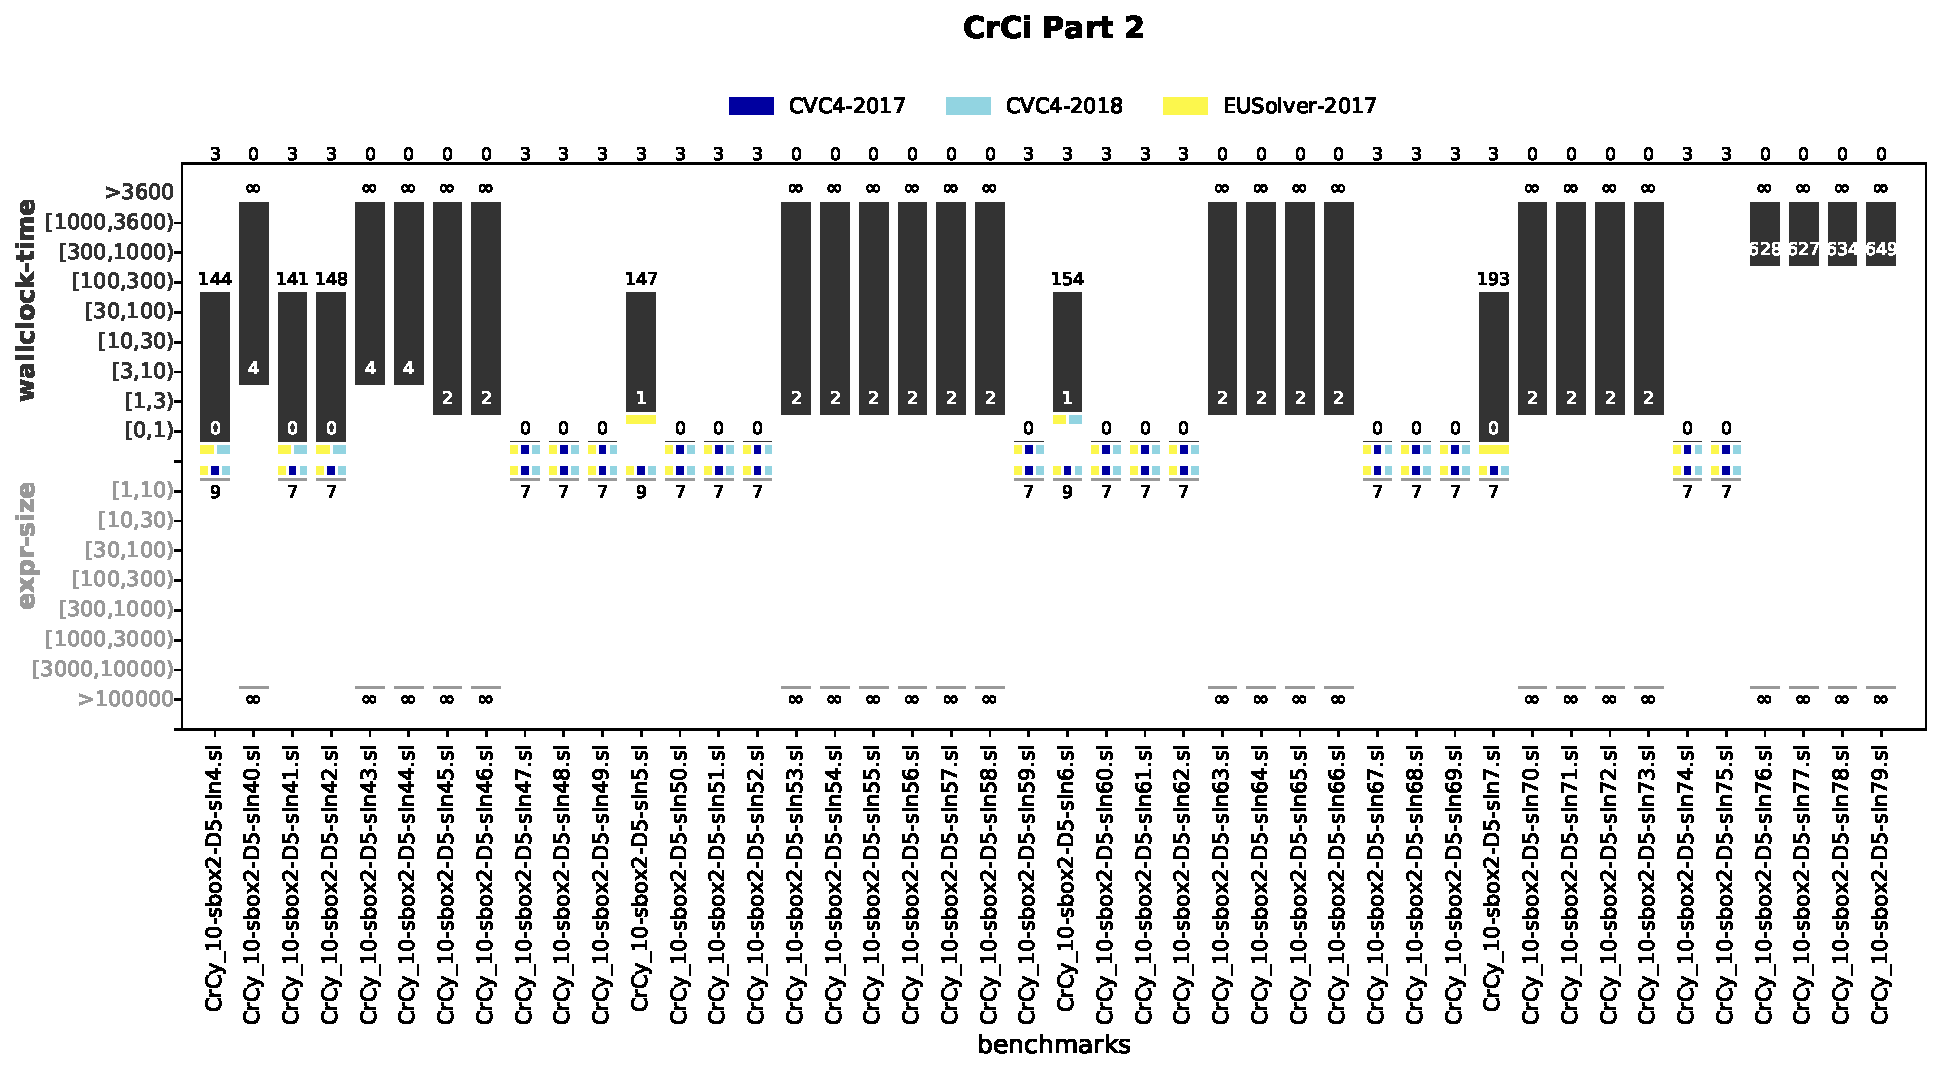
\includegraphics[width=10in]{figures/CrCi2.pdf}
			\end{tabular}
	}}
	\caption{Evaluation of crypto circuits category of the General track (Parts 1 \& 2).}
	\label{fig:crci-1}
\end{figure*}

\begin{figure*}
	\noindent\makebox[\textwidth]{
		\scalebox{0.625}{
			\begin{tabular}{c}
				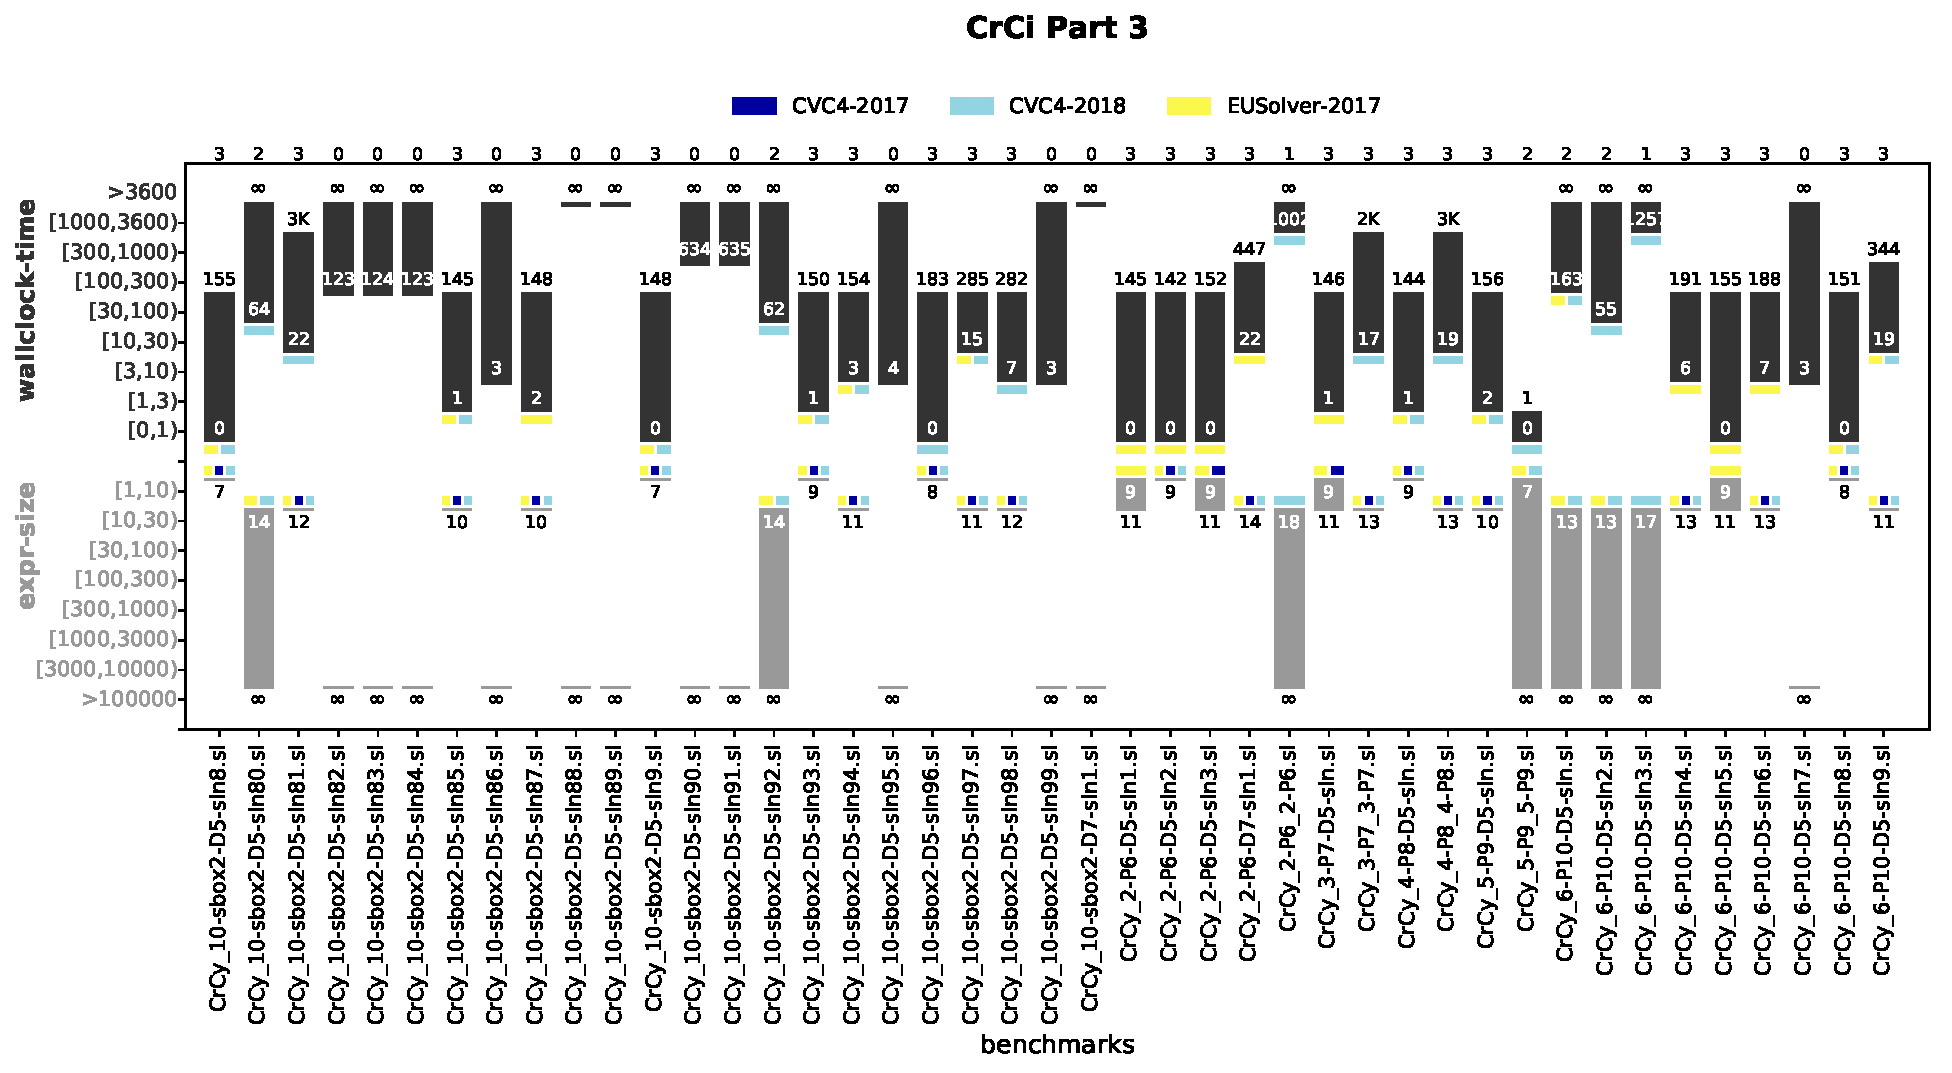
\includegraphics[width=10in]{figures/CrCi3.pdf} \\[3cm]
				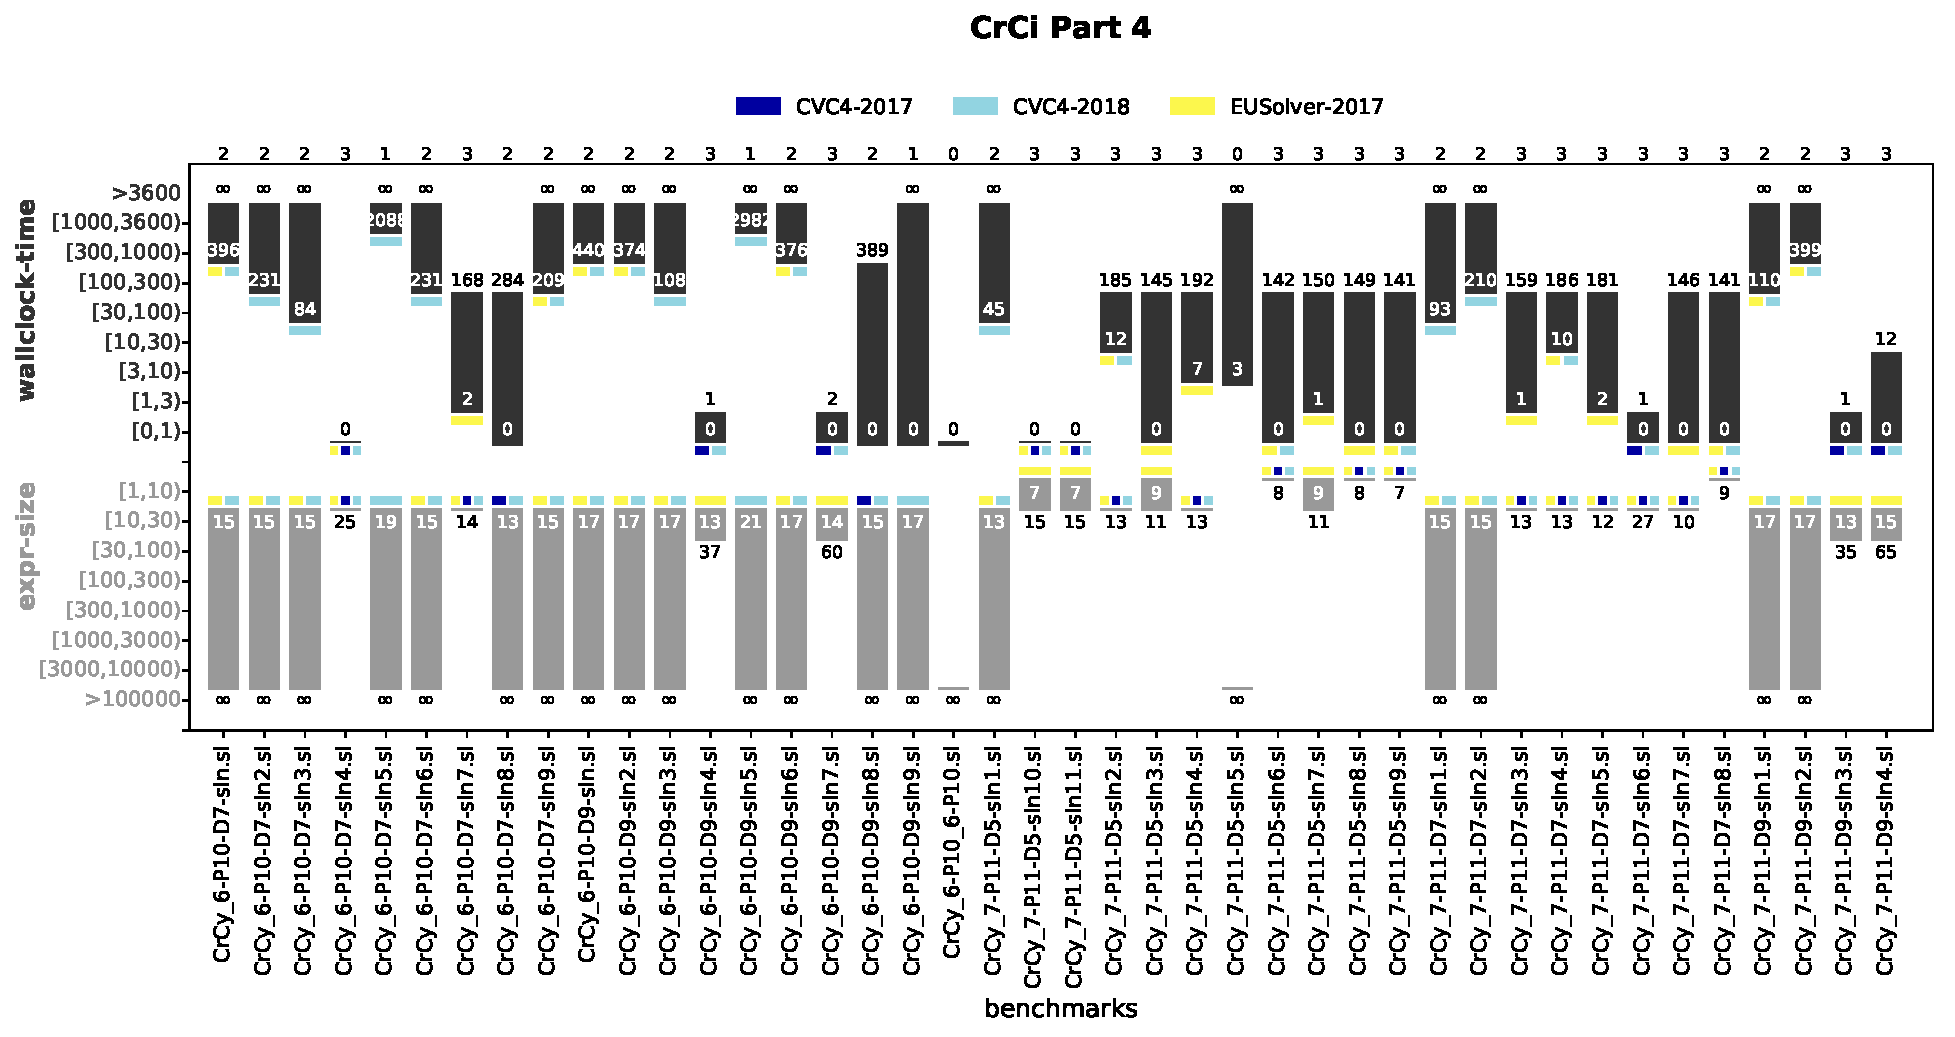
\includegraphics[width=10in]{figures/CrCi4.pdf}
			\end{tabular}
	}}
	\caption{Evaluation of crypto circuits category of the General track (Parts 3 \& 4).}
	\label{fig:crci-2}
\end{figure*}
	
\begin{figure*}
	\noindent\makebox[\textwidth]{
		\scalebox{0.625}{
			\begin{tabular}{c}
				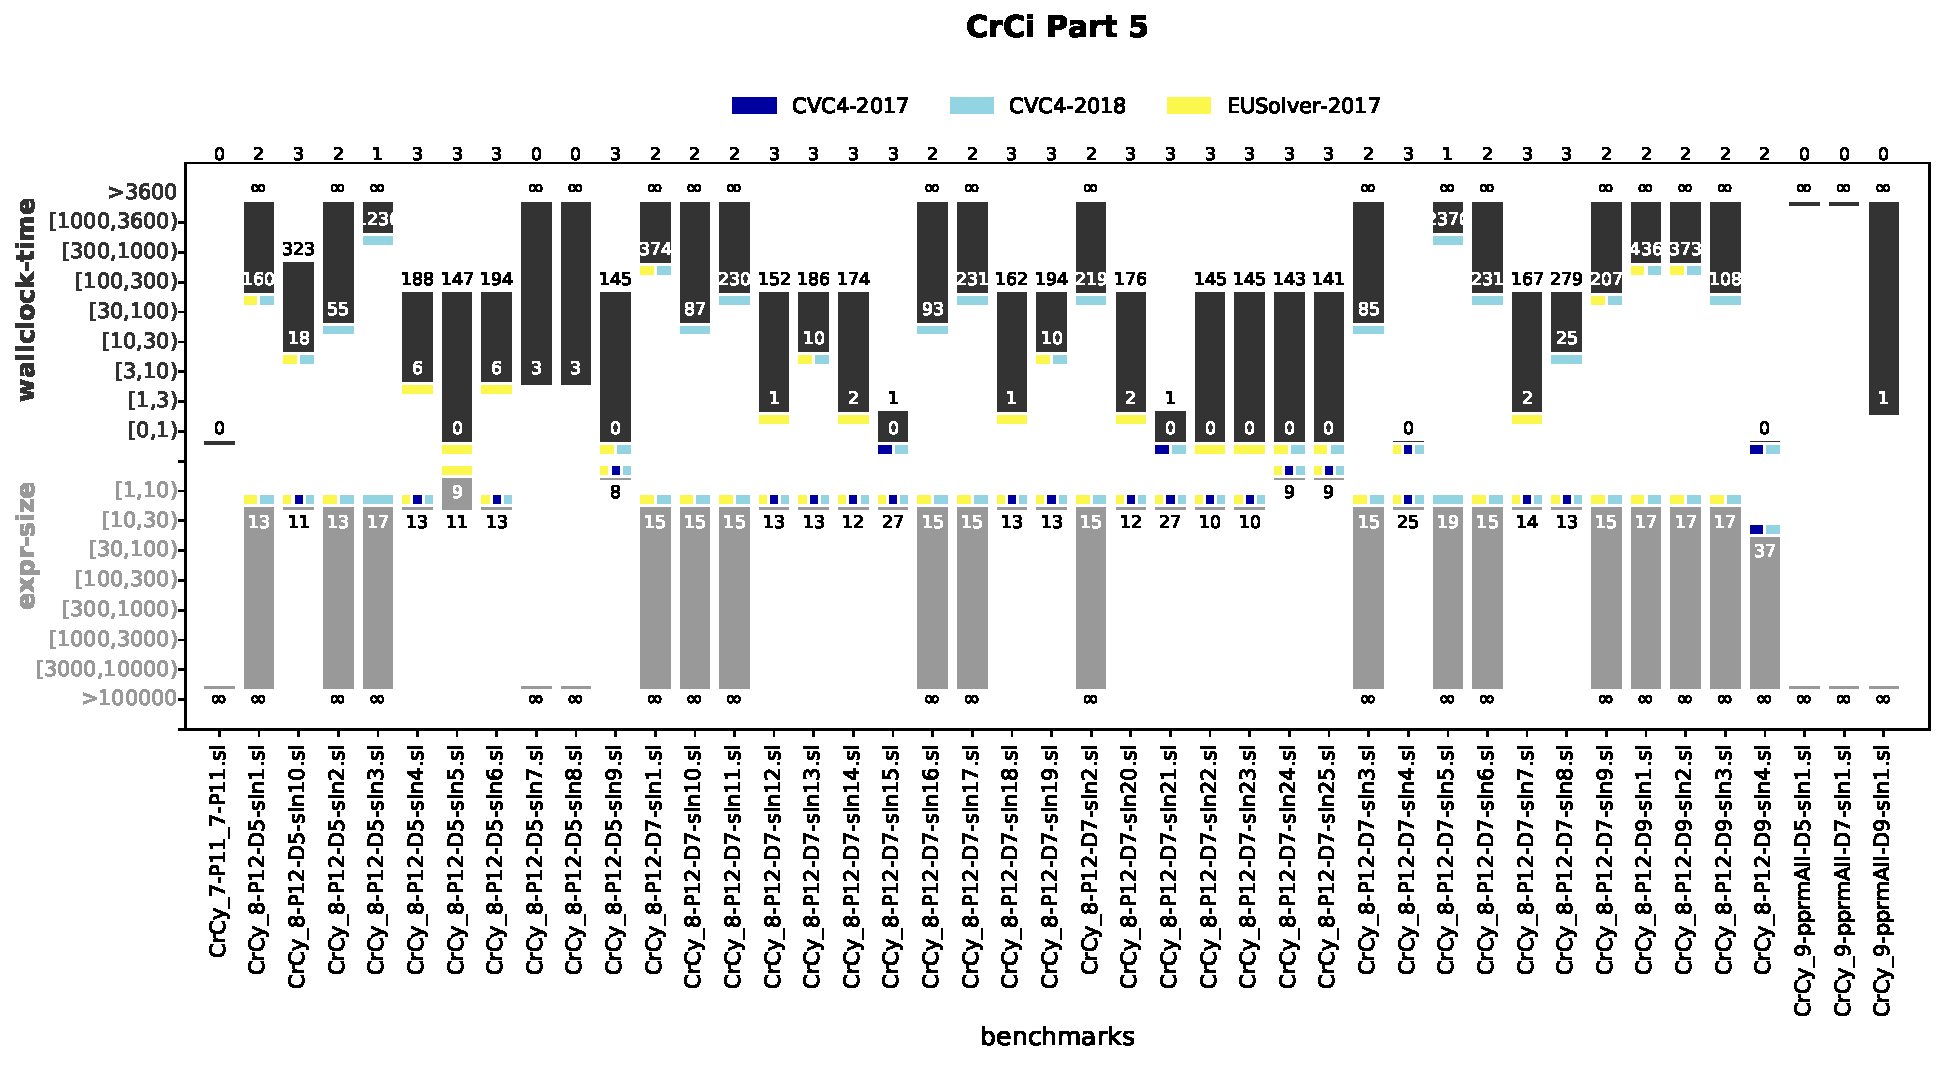
\includegraphics[width=10in]{figures/CrCi5.pdf}
			\end{tabular}
	}}
	\caption{Evaluation of crypto circuits category of the General track (Part 5).}
	\label{fig:crci-5}
\end{figure*}
	

\begin{figure*}
	\noindent\makebox[\textwidth]{
		\scalebox{0.6}{
			\begin{tabular}{c}
				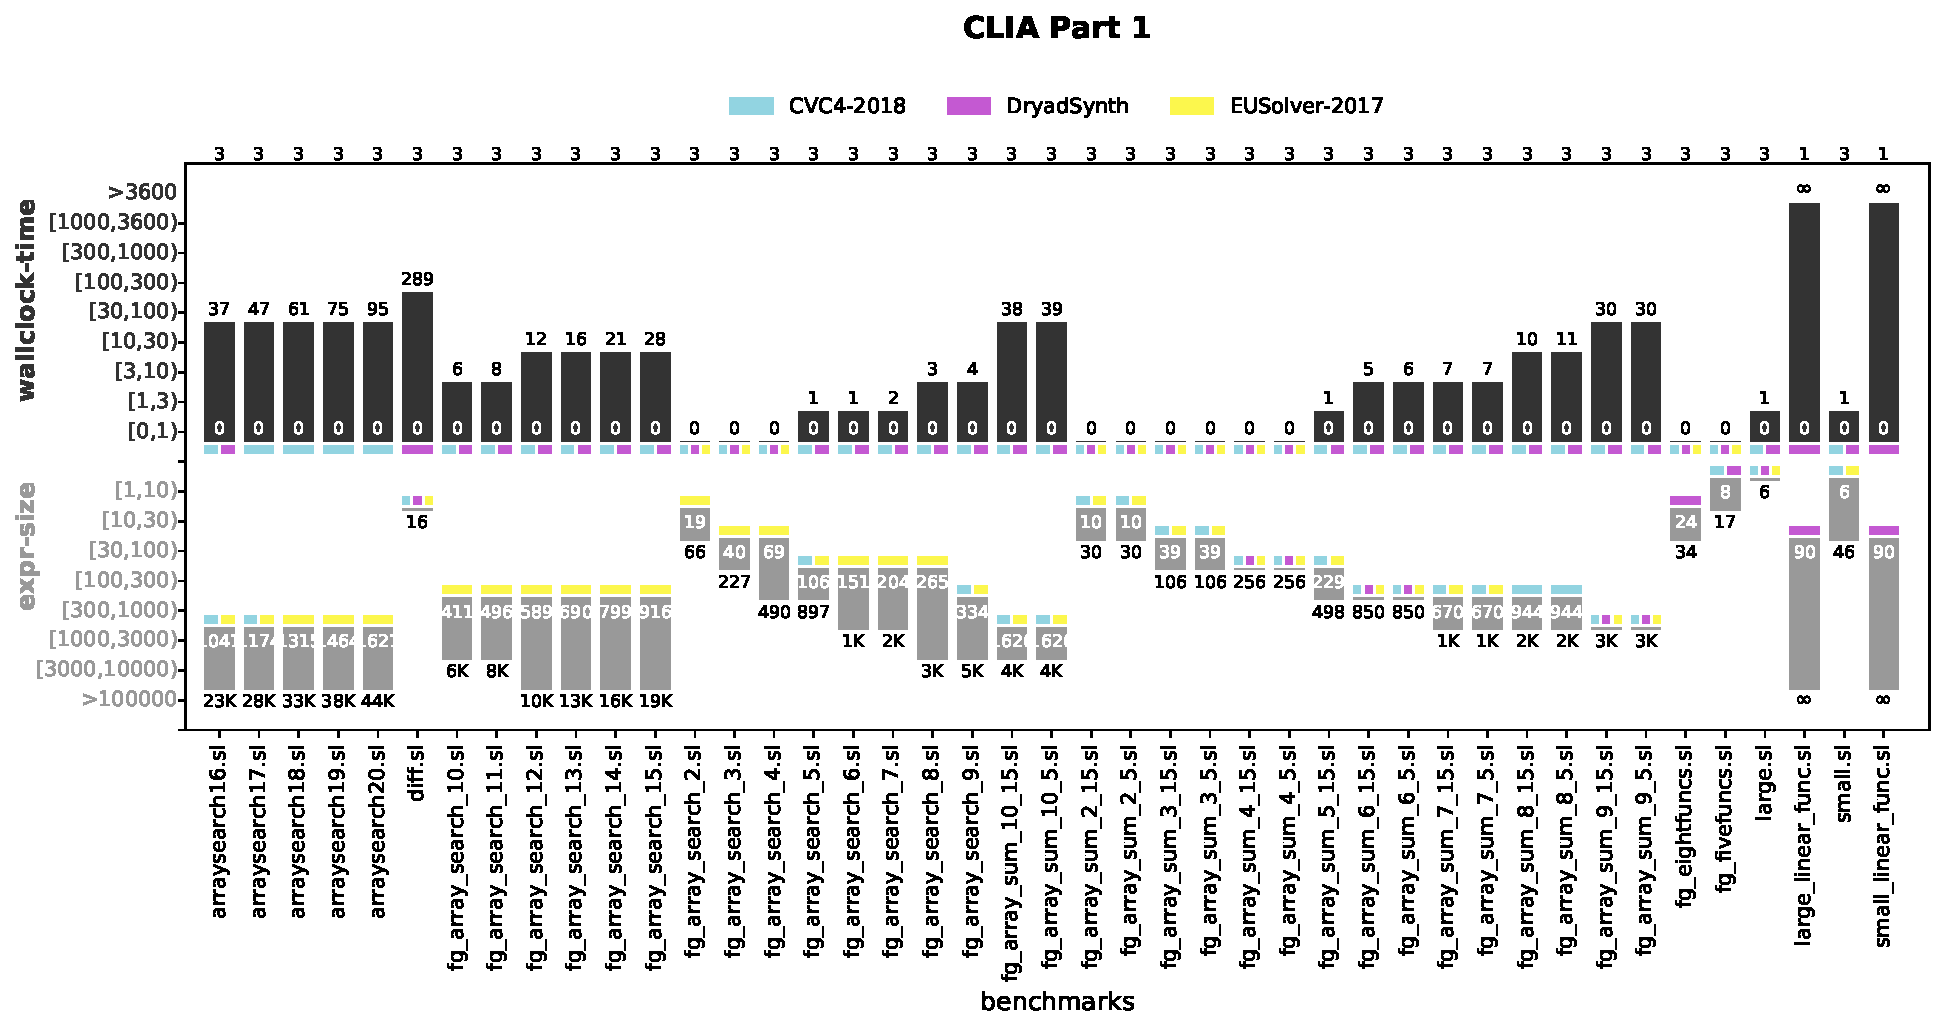
\includegraphics[width=10in]{figures/CLIA1.pdf} \\[3cm]
				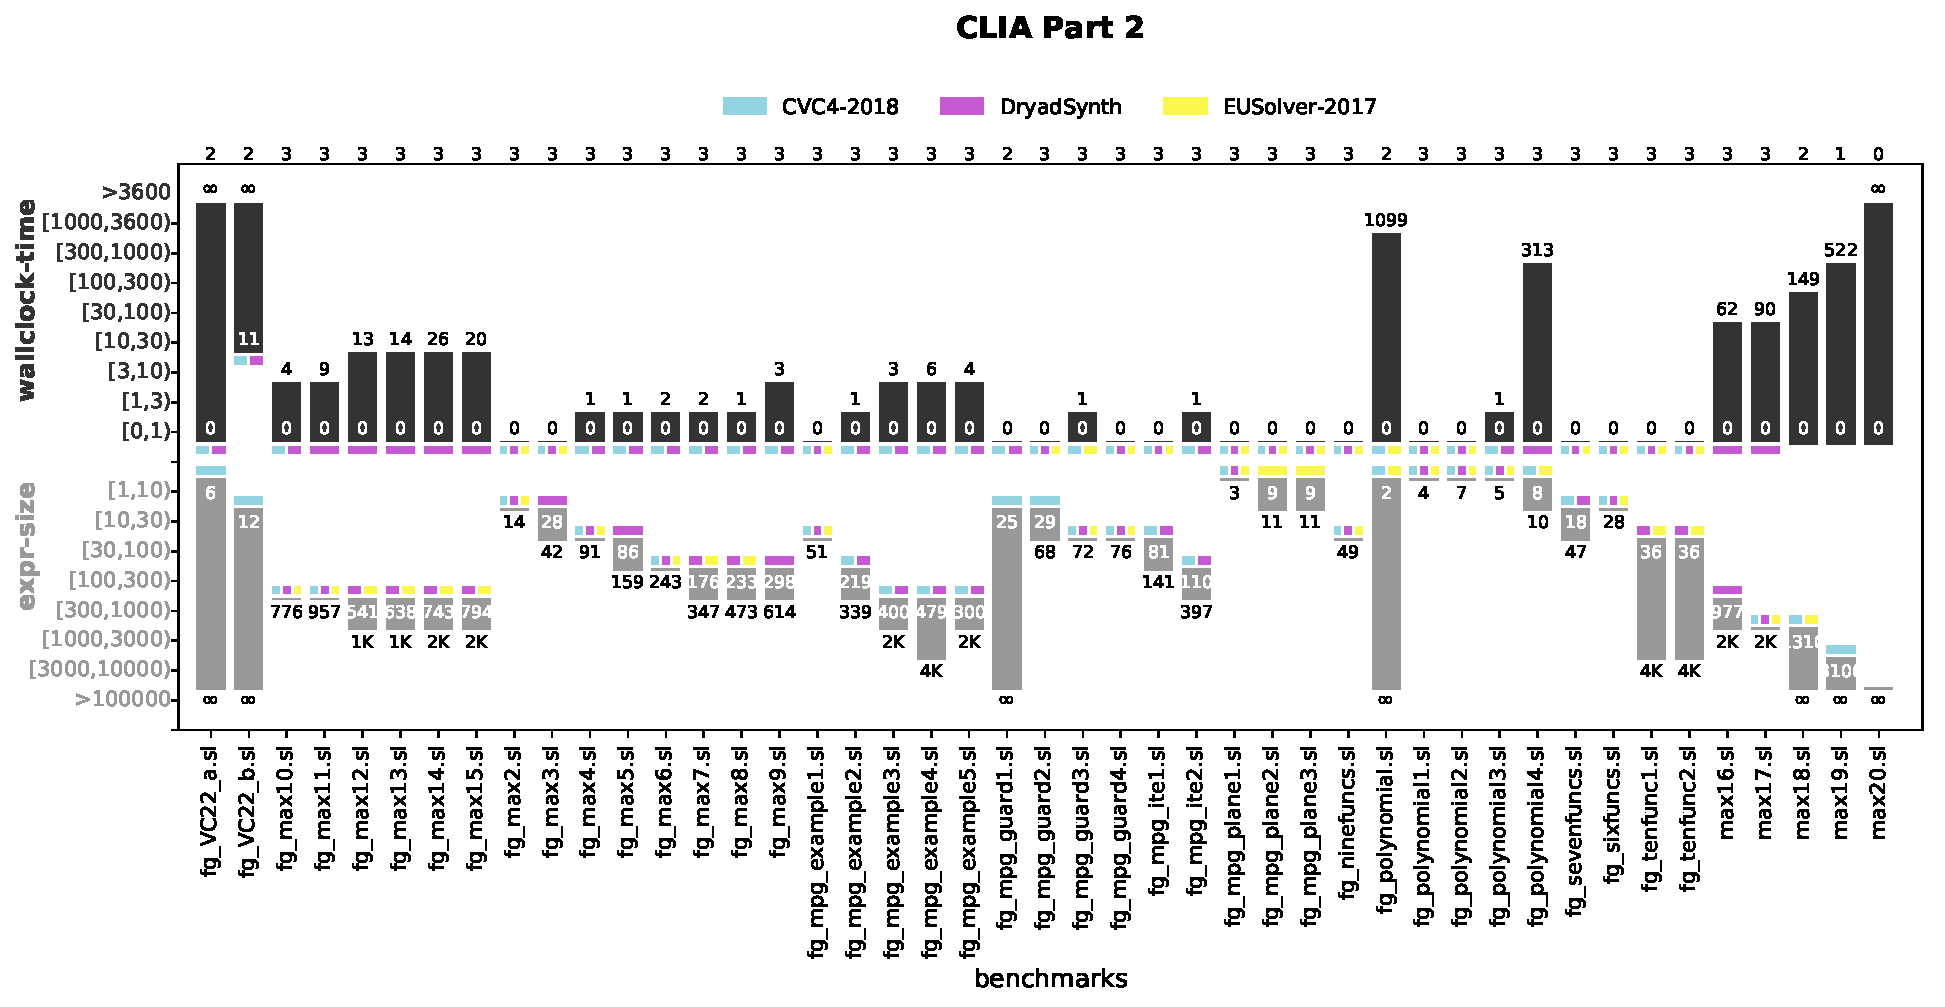
\includegraphics[width=10in]{figures/CLIA2.pdf} 
			\end{tabular}
	}}
	\caption{Evaluation of CLIA track benchmarks.}
	\label{fig:clia-results}
\end{figure*}



\begin{figure*}
	\noindent\makebox[\textwidth]{
		\scalebox{0.6}{
			\begin{tabular}{c}
				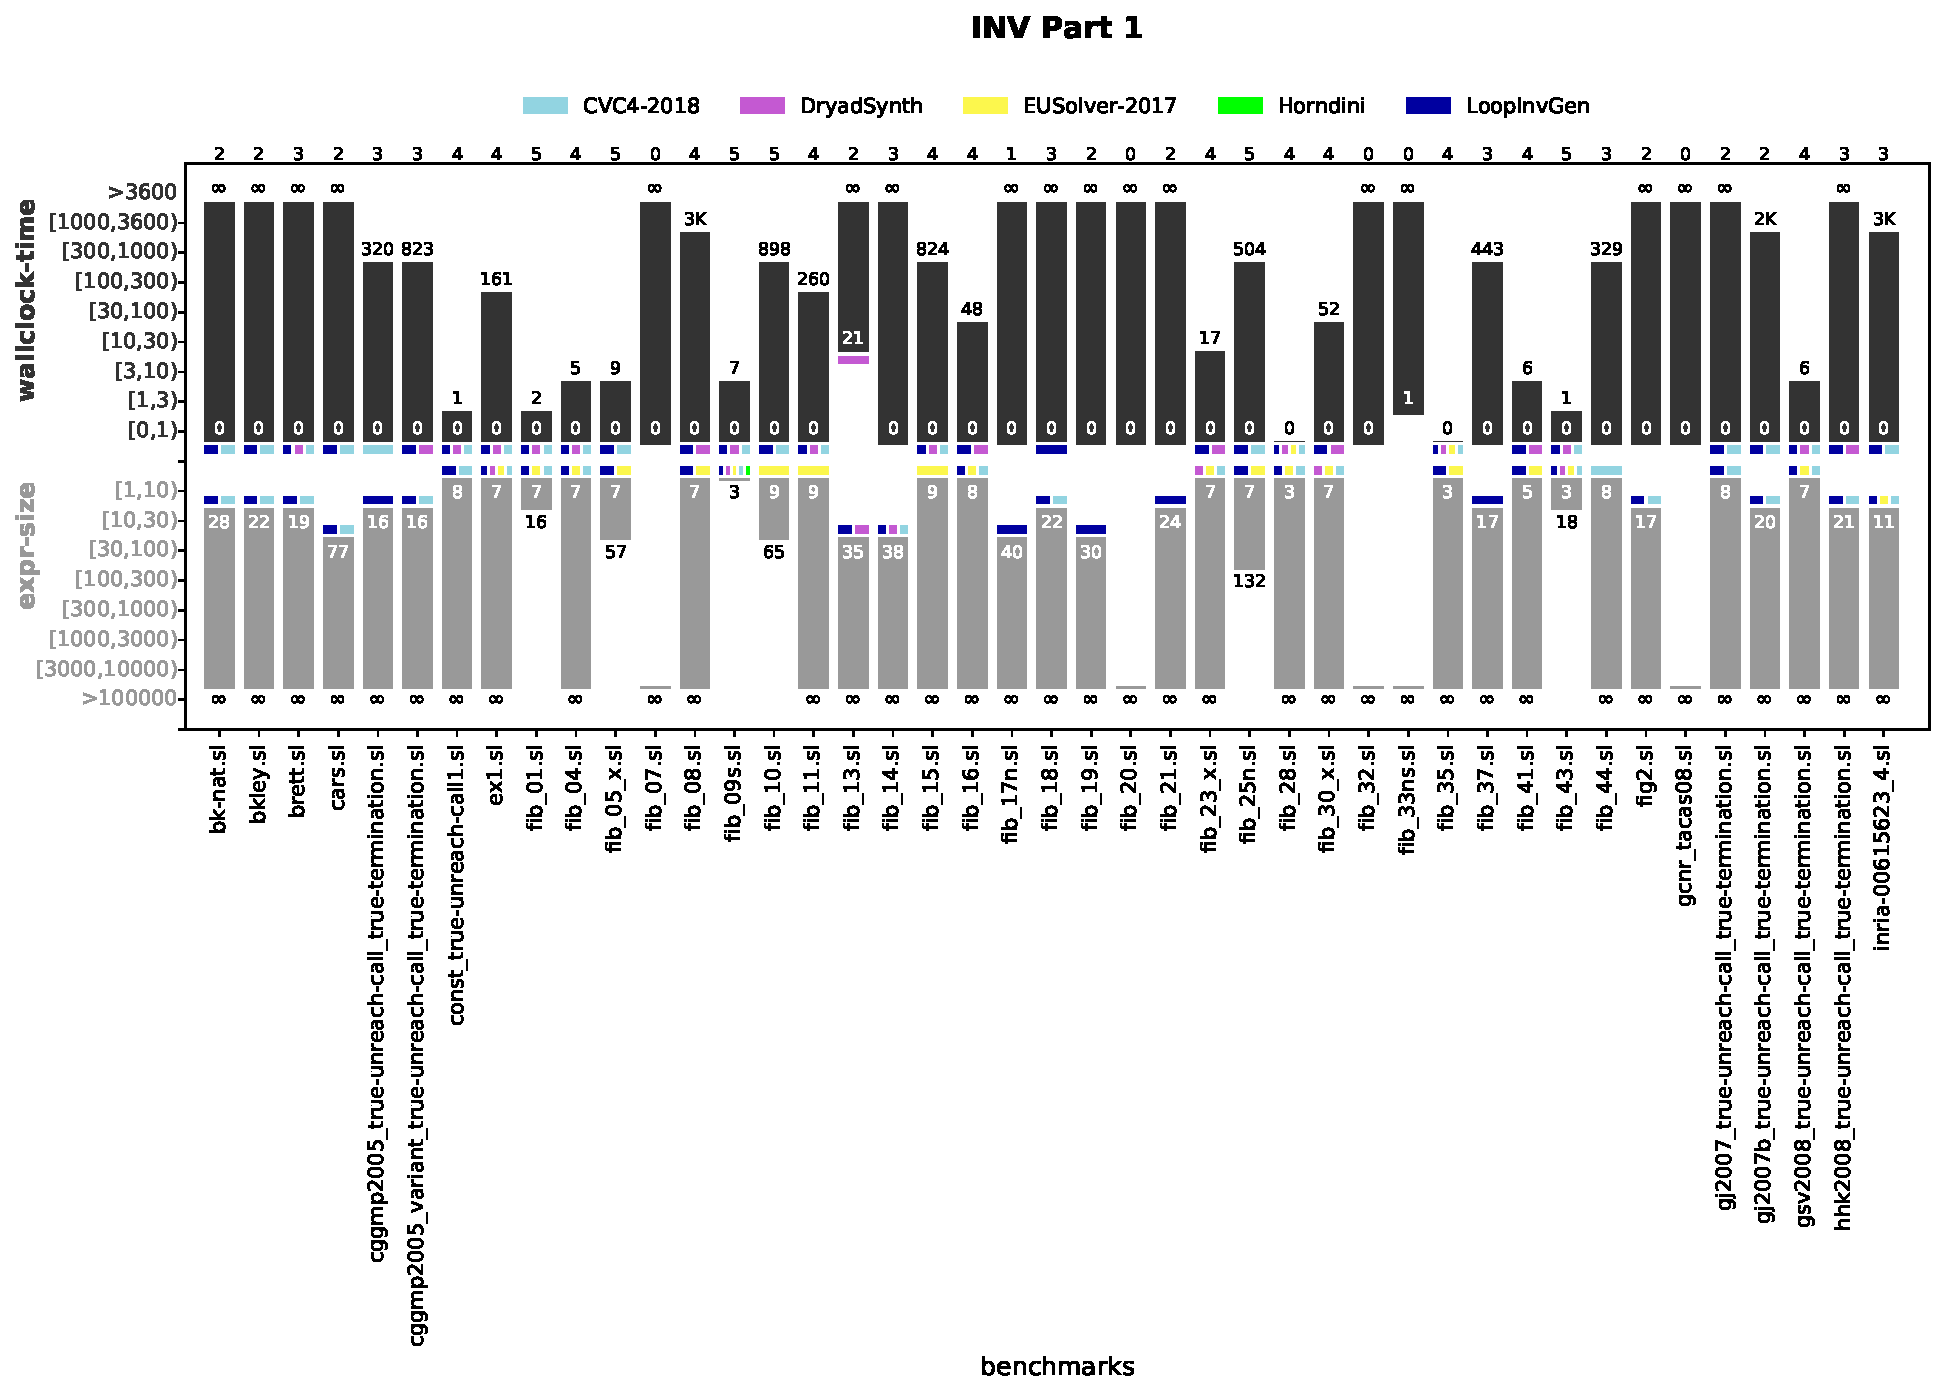
\includegraphics[width=10in]{figures/Inv1.pdf} \\[5mm]
				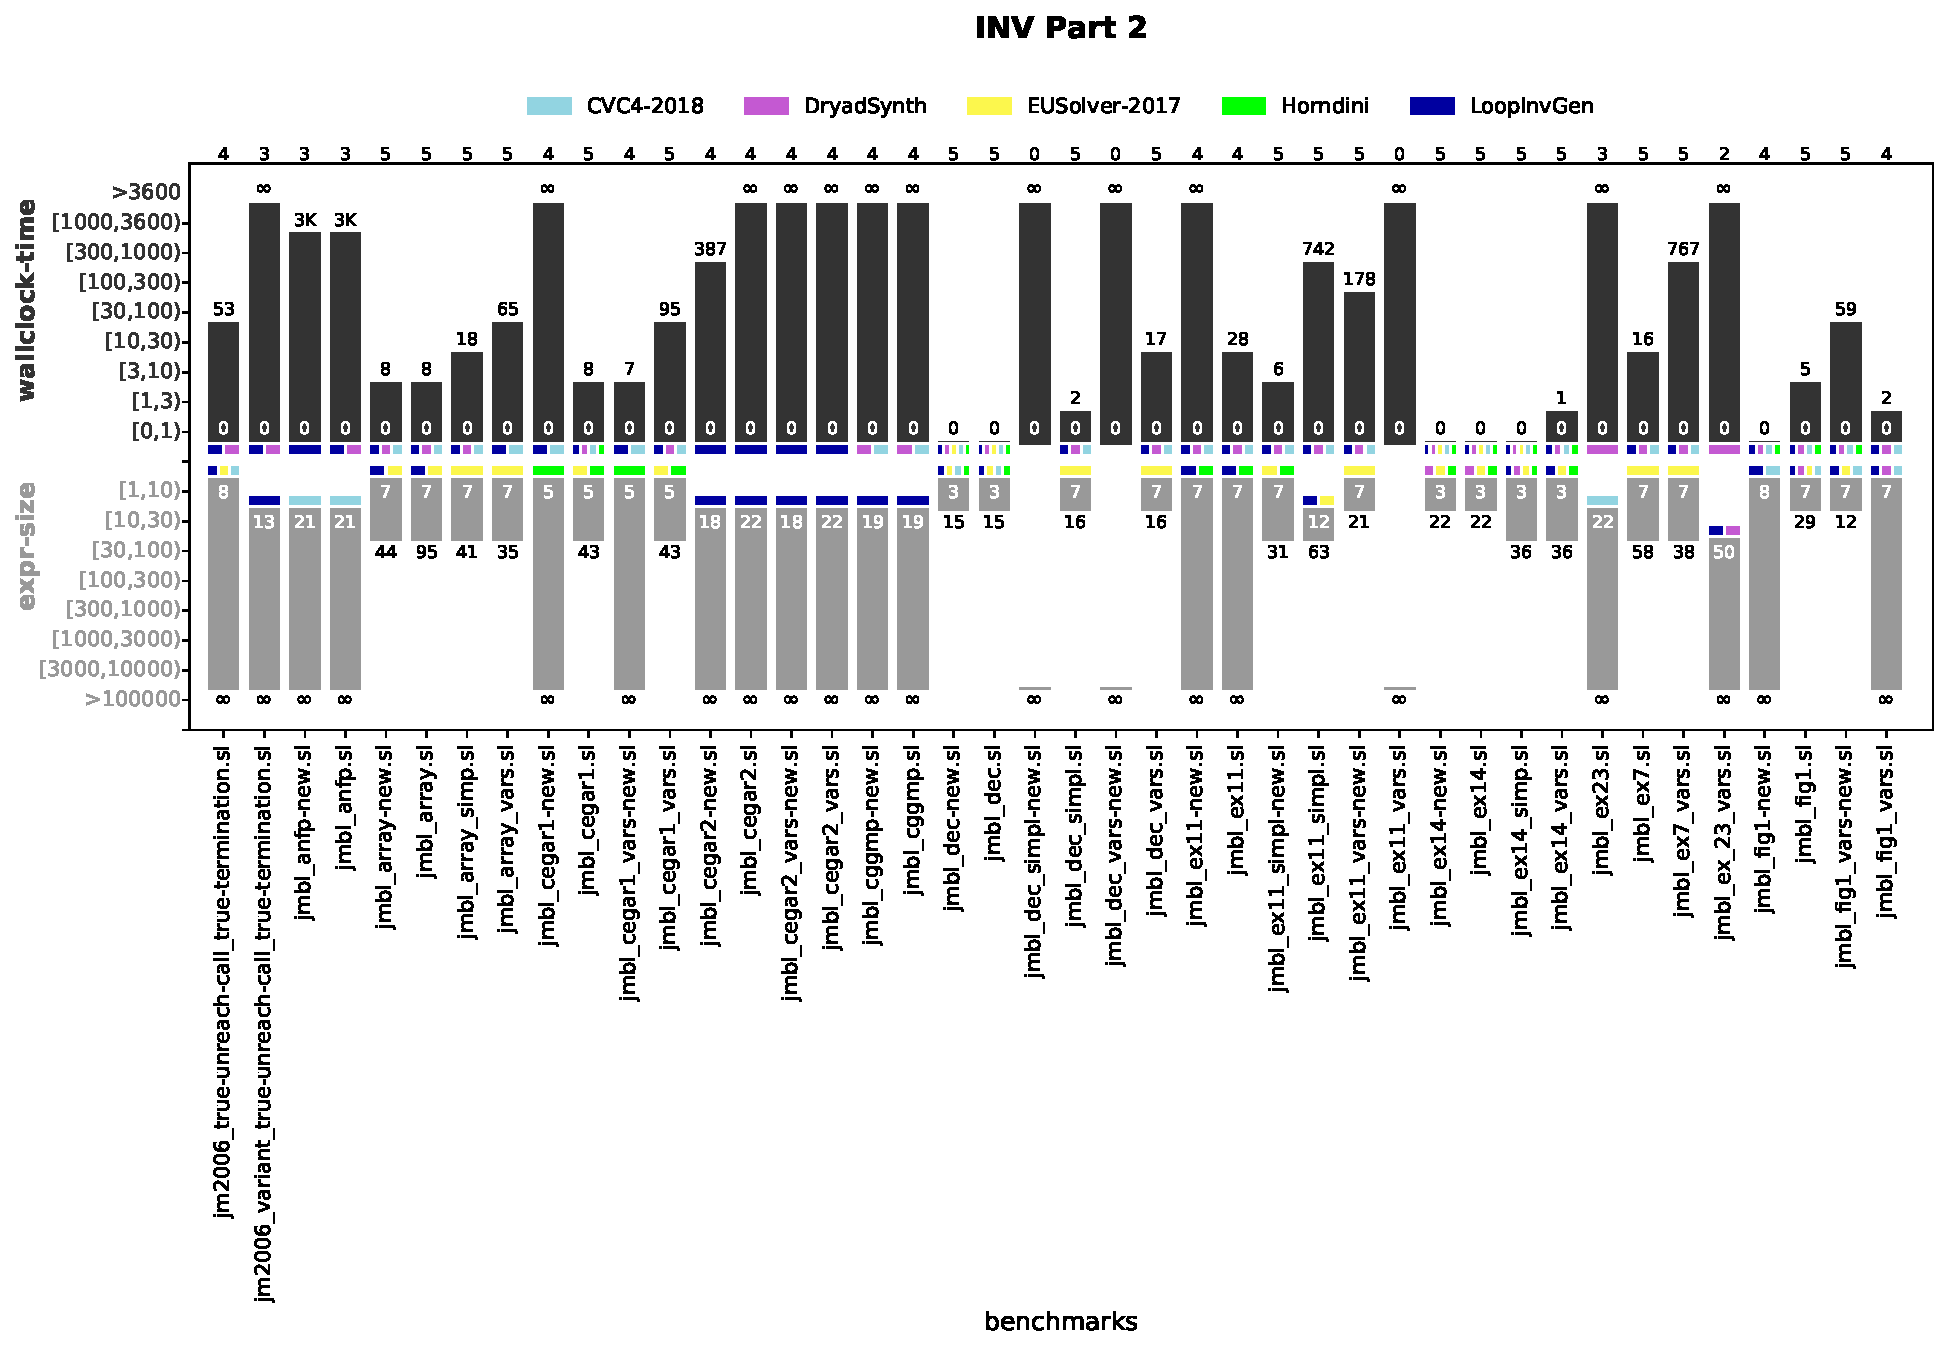
\includegraphics[width=10in]{figures/Inv2.pdf}
			\end{tabular}
	}}
	\caption{Evaluation of Invariant track benchmarks (Parts 1 \& 2).}
	\label{fig:inv-results-1}
\end{figure*}



\begin{figure*}
	\noindent\makebox[\textwidth]{
		\scalebox{0.6}{
			\begin{tabular}{c}
				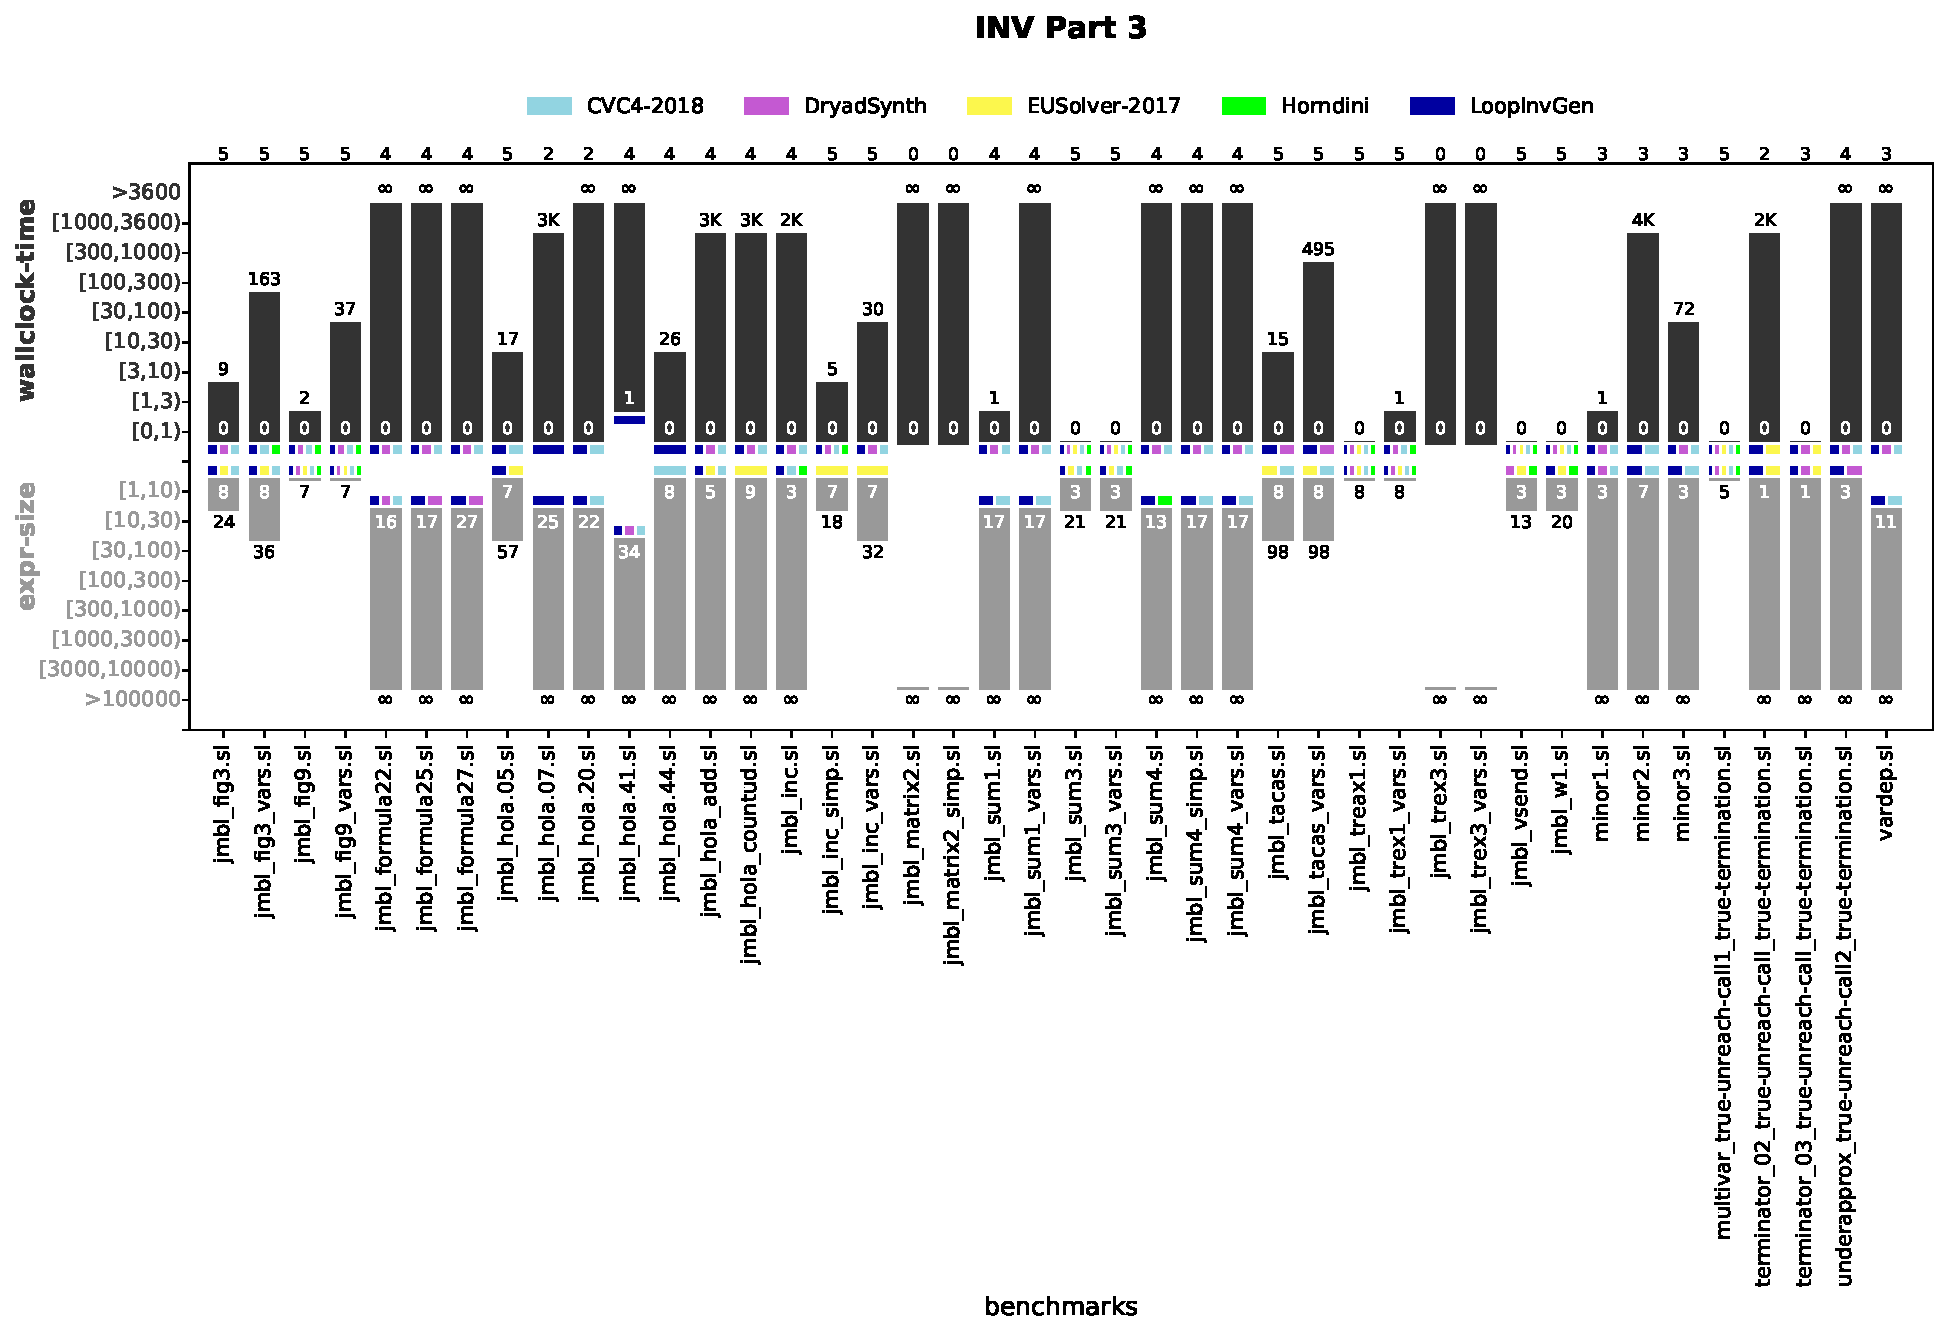
\includegraphics[width=10in]{figures/Inv3.pdf}
			\end{tabular}
		}}
	\caption{Evaluation of Invariant track benchmarks (Part 3).}
	\label{fig:inv-results-2}
\end{figure*}

\begin{figure*}
	\noindent\makebox[\textwidth]{
		\scalebox{0.6}{
			\begin{tabular}{c}
				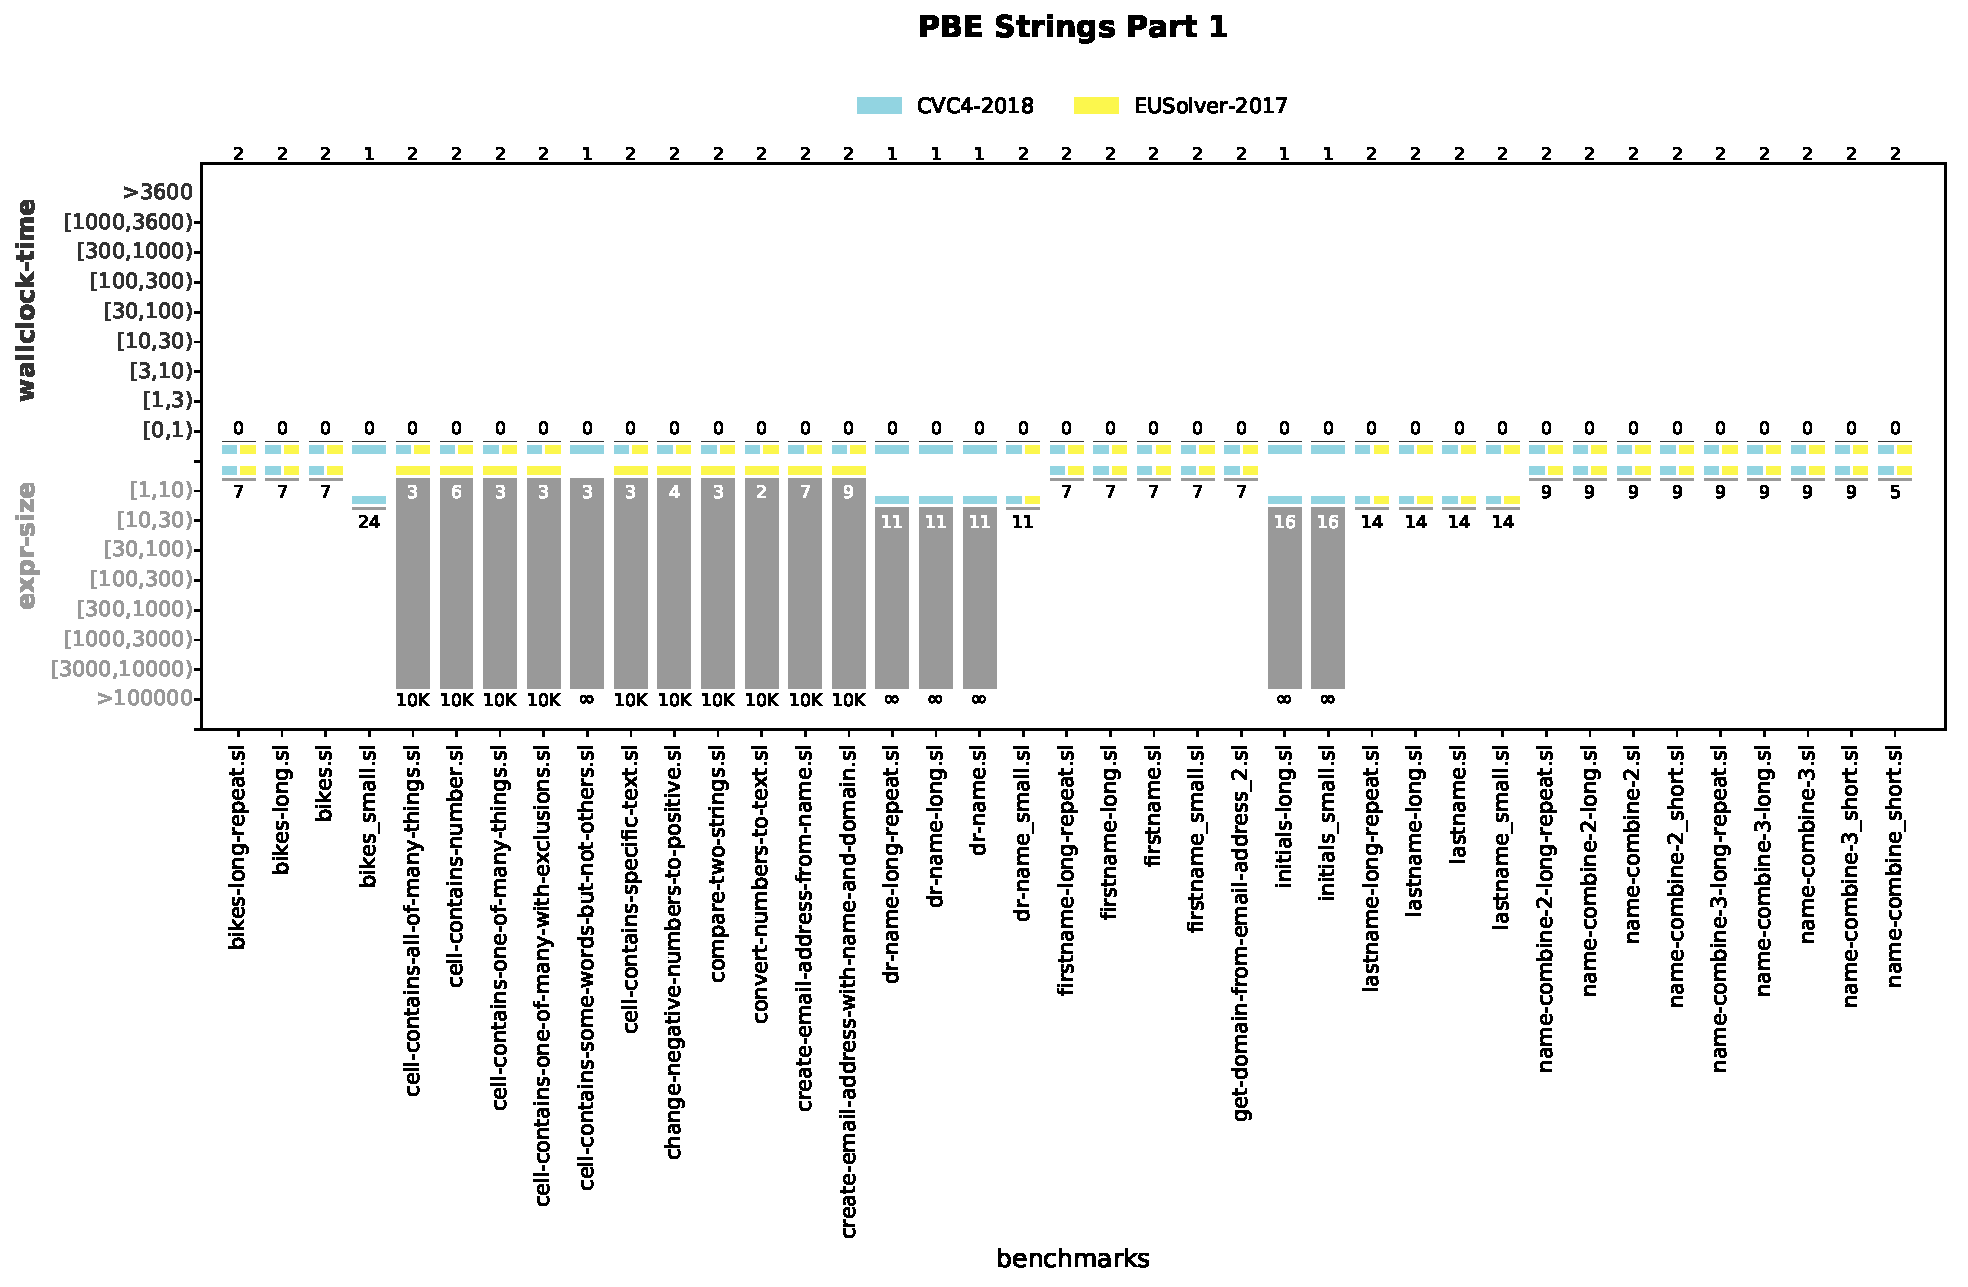
\includegraphics[width=10in]{figures/PBEStrings1.pdf} \\[3cm]
				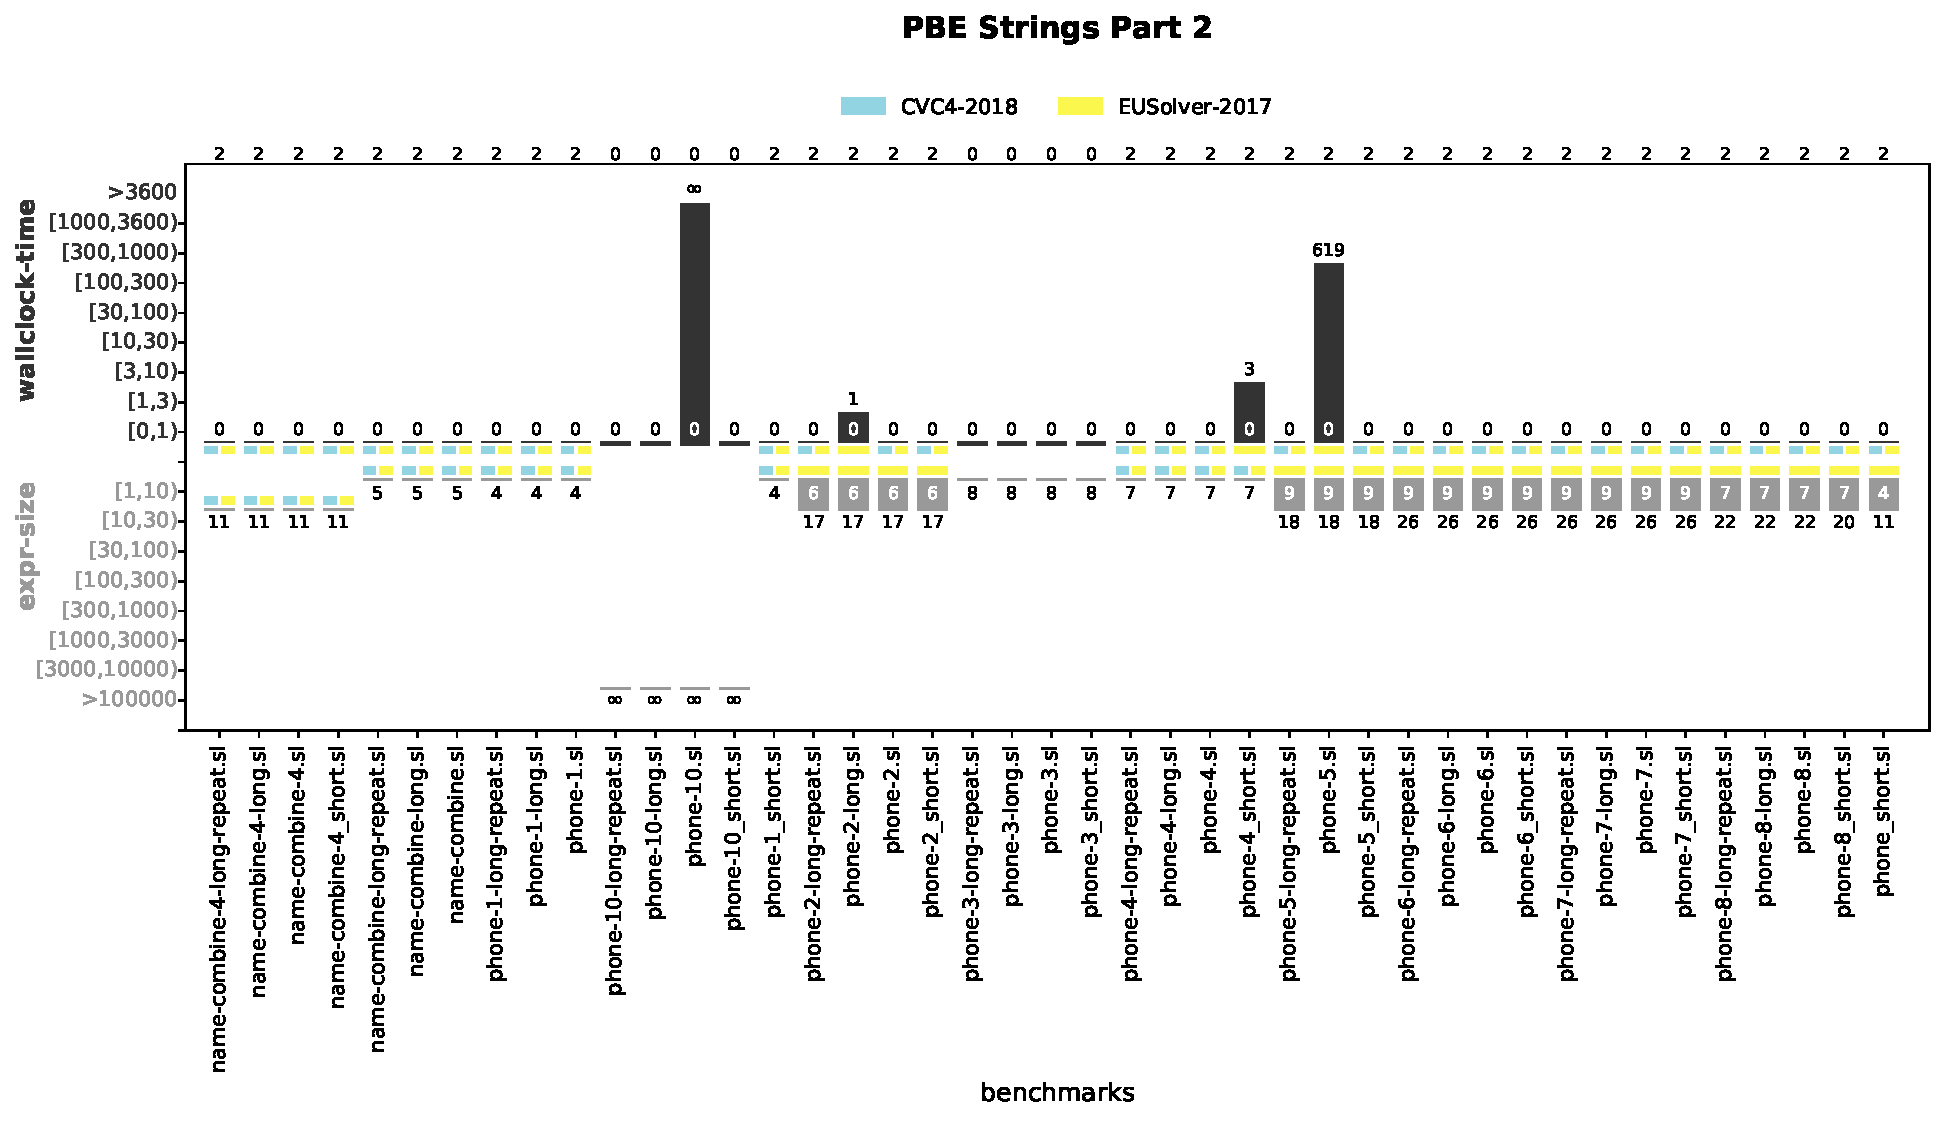
\includegraphics[width=10in]{figures/PBEStrings2.pdf} 
			\end{tabular}
		}}
	\caption{Evaluation of PBE Strings track benchmarks.}
	\label{fig:pbe-strings-results}
\end{figure*}